% Options for packages loaded elsewhere
\PassOptionsToPackage{unicode}{hyperref}
\PassOptionsToPackage{hyphens}{url}
\PassOptionsToPackage{dvipsnames,svgnames,x11names}{xcolor}
%
\documentclass[
  12pt,
  twoside,
  openright,
  a4paper,
  chapter=TITLE,
  section=TITLE,
  brazil]{abntex2}

\usepackage{amsmath,amssymb}
\usepackage{iftex}
\ifPDFTeX
  \usepackage[T1]{fontenc}
  \usepackage[utf8]{inputenc}
  \usepackage{textcomp} % provide euro and other symbols
\else % if luatex or xetex
  \usepackage{unicode-math}
  \defaultfontfeatures{Scale=MatchLowercase}
  \defaultfontfeatures[\rmfamily]{Ligatures=TeX,Scale=1}
\fi
\usepackage{lmodern}
\ifPDFTeX\else  
    % xetex/luatex font selection
\fi
% Use upquote if available, for straight quotes in verbatim environments
\IfFileExists{upquote.sty}{\usepackage{upquote}}{}
\IfFileExists{microtype.sty}{% use microtype if available
  \usepackage[]{microtype}
  \UseMicrotypeSet[protrusion]{basicmath} % disable protrusion for tt fonts
}{}
\makeatletter
\@ifundefined{KOMAClassName}{% if non-KOMA class
  \IfFileExists{parskip.sty}{%
    \usepackage{parskip}
  }{% else
    \setlength{\parindent}{0pt}
    \setlength{\parskip}{6pt plus 2pt minus 1pt}}
}{% if KOMA class
  \KOMAoptions{parskip=half}}
\makeatother
\usepackage{xcolor}
\setlength{\emergencystretch}{3em} % prevent overfull lines
\setcounter{secnumdepth}{5}
% Make \paragraph and \subparagraph free-standing
\ifx\paragraph\undefined\else
  \let\oldparagraph\paragraph
  \renewcommand{\paragraph}[1]{\oldparagraph{#1}\mbox{}}
\fi
\ifx\subparagraph\undefined\else
  \let\oldsubparagraph\subparagraph
  \renewcommand{\subparagraph}[1]{\oldsubparagraph{#1}\mbox{}}
\fi


\providecommand{\tightlist}{%
  \setlength{\itemsep}{0pt}\setlength{\parskip}{0pt}}\usepackage{longtable,booktabs,array}
\usepackage{calc} % for calculating minipage widths
% Correct order of tables after \paragraph or \subparagraph
\usepackage{etoolbox}
\makeatletter
\patchcmd\longtable{\par}{\if@noskipsec\mbox{}\fi\par}{}{}
\makeatother
% Allow footnotes in longtable head/foot
\IfFileExists{footnotehyper.sty}{\usepackage{footnotehyper}}{\usepackage{footnote}}
\makesavenoteenv{longtable}
\usepackage{graphicx}
\makeatletter
\def\maxwidth{\ifdim\Gin@nat@width>\linewidth\linewidth\else\Gin@nat@width\fi}
\def\maxheight{\ifdim\Gin@nat@height>\textheight\textheight\else\Gin@nat@height\fi}
\makeatother
% Scale images if necessary, so that they will not overflow the page
% margins by default, and it is still possible to overwrite the defaults
% using explicit options in \includegraphics[width, height, ...]{}
\setkeys{Gin}{width=\maxwidth,height=\maxheight,keepaspectratio}
% Set default figure placement to htbp
\makeatletter
\def\fps@figure{htbp}
\makeatother

% opções para o classoption
%
%	12pt,				% tamanho da fonte
%	openright,			% capítulos começam em pág ímpar (insere página vazia caso preciso)
%	twoside,			% para impressão em recto e verso. Oposto a oneside
%	a4paper,			% tamanho do papel. 
%	% -- opções da classe abntex2 --
%	%chapter=TITLE,		% títulos de capítulos convertidos em letras maiúsculas
%	%section=TITLE,		% títulos de seções convertidos em letras maiúsculas
%	%subsection=TITLE,	% títulos de subseções convertidos em letras maiúsculas
%	%subsubsection=TITLE,% títulos de subsubseções convertidos em letras maiúsculas
%	% -- opções do pacote babel --
%	english,			% idioma adicional para hifenização
%	french,				% idioma adicional para hifenização
%	spanish,			% idioma adicional para hifenização
%	brazil				% o último idioma é o principal do documento

% ---
% Pacotes básicos 
% ---
\usepackage{lmodern}			% Usa a fonte Latin Modern			
\usepackage[T1]{fontenc}		% Selecao de codigos de fonte.
\usepackage[utf8]{inputenc}		% Codificacao do documento (conversão automática dos acentos)
\usepackage{indentfirst}		% Indenta o primeiro parágrafo de cada seção.
\usepackage{color}				% Controle das cores
\usepackage{graphicx}			% Inclusão de gráficos
\usepackage{microtype} 			% para melhorias de justificação
\usepackage{config/tema/ppgecotex}	% customização para PPGEco/UFES
% ---

% ---
% Pacotes adicionais
% ---
\usepackage{lipsum}																% para geração de dummy text
\usepackage{bbm, times, quoting, setspace, lscape}
\usepackage{psfrag, fancyhdr}
\usepackage{amsmath, amsfonts, amssymb, amsthm}									% escrita matemática
\usepackage{xcolor, url, placeins, enumitem}
\usepackage{dcolumn, lastpage, listings}
\usepackage[skip = 2pt, size = normalsize, labelfont = bf]{caption}
\usepackage[portuguese, ruled, lined]{algorithm2e}

% ---

% ---
% Pacotes de citações
% ---
\usepackage[backend=biber, style=abnt, justify, giveninits, backref=true, backrefstyle=three, citecounter=true]{biblatex}

% fontes
\setmainfont{Times New Roman}
\setmonofont[Scale=0.9, Scale=MatchLowercase]{Consolas}

% teoremas
\newtheorem{theorem}{Teorema}[chapter]
\newtheorem{proposition}{Proposição}[chapter]
\newtheorem{lemma}[theorem]{Lema}
\newtheorem{corollary}{Corolário}[theorem]

% --- 
% CONFIGURAÇÕES DE PACOTES
% --- 

% ---
% Configurações de aparência do PDF final

% alterando o aspecto da cor azul
\definecolor{blue}{RGB}{41,5,195}

% informações do PDF
\makeatletter
\hypersetup{
     	%pagebackref=true,
		pdftitle={\@title}, 
		pdfauthor={\@author},
    	pdfsubject={\imprimirpreambulo},
	    pdfcreator={LaTeX with abnTeX2},
		pdfkeywords={séries temporais hierárquicas}{economia bancária}{machine learning}{abntex2}{trabalho acadêmico}, 
		colorlinks=true,       		% false: boxed links; true: colored links
    	linkcolor=blue,          	% color of internal links
    	citecolor=blue,        		% color of links to bibliography
    	filecolor=magenta,      		% color of file links
		urlcolor=blue,
		bookmarksdepth=4
}
\makeatother
% --- 

% ---
% Posiciona figuras e tabelas no topo da página quando adicionadas sozinhas
% em um página em branco. Ver https://github.com/abntex/abntex2/issues/170
\makeatletter
\setlength{\@fptop}{5pt} % Set distance from top of page to first float
\makeatother
% ---

% ---
% Possibilita criação de Quadros e Lista de quadros.
% Ver https://github.com/abntex/abntex2/issues/176
%
\newcommand{\quadroname}{Quadro}
\newcommand{\listofquadrosname}{Lista de Quadros}

\newfloat[chapter]{quadro}{loq}{\quadroname}
\newlistof{listofquadros}{loq}{\listofquadrosname}
\newlistentry{quadro}{loq}{0}

% configurações para atender às regras da ABNT
\setfloatadjustment{quadro}{\centering}
\counterwithout{quadro}{chapter}
\renewcommand{\cftquadroname}{\quadroname\space} 
\renewcommand*{\cftquadroaftersnum}{\hfill--\hfill}

\setfloatlocations{quadro}{hbtp} % Ver https://github.com/abntex/abntex2/issues/176
% ---

% --- 
% Espaçamentos entre linhas e parágrafos 
% --- 

% O tamanho do parágrafo é dado por:
\setlength{\parindent}{1.3cm}

% Controle do espaçamento entre um parágrafo e outro:
\setlength{\parskip}{0.2cm}  % tente também \onelineskip

% ---
% compila o indice
% ---
\makeindex
% ---

% Seleciona o idioma do documento (conforme pacotes do babel)
%\selectlanguage{english}
\selectlanguage{brazil}
\captionsetup[figure]{name=Figura}
\captionsetup[table]{name=Tabela}

% Retira espaço extra obsoleto entre as frases.
\frenchspacing 

% matrizes
\setcounter{MaxMatrixCols}{20}

% bibliografia
\addbibresource{config/elementos/dissertacao.bib}
\addbibresource{config/elementos/packages.bib}

% fazer sumário começar do 1 ao invés do zero
\renewcommand{\thesection}{\arabic{section}}

% posição das figuras
\setfloatlocations{figure}{hbtp}
\setfloatlocations{table}{hbtp}

% code snippets
\lstset{language=R,
    basicstyle=\small\ttfamily,
    stringstyle=\color{DarkGreen},
    otherkeywords={0,1,2,3,4,5,6,7,8,9},
    morekeywords={TRUE,FALSE},
    deletekeywords={data,frame,length,as,character},
    keywordstyle=\color{blue},
    commentstyle=\color{DarkGreen},
	showstringspaces=false
}
\titulo{MÉTODOS DE MACHINE LEARNING PARA RECONCILIAÇÃO ÓTIMA DE SÉRIES TEMPORAIS HIERÁRQUICAS E AGRUPADAS DE INSTITUIÇÕES FINANCEIRAS}
\local{VITÓRIA}
\orientador{Prof. Dr. Guilherme A. de A. Pereira}
\instituicao{%
    UNIVERSIDADE FEDERAL DO ESPÍRITO SANTO
    \par
    CENTRO DE CIÊNCIAS JURÍDICAS E ECONÔMICAS
    \par
    PROGRAMA DE PÓS-GRADUAÇÃO EM ECONOMIA}
\tipotrabalho{Dissertação (Mestrado)}
\preambulo{Dissertação apresentada ao Programa de Pós-Graduação em Economia da Universidade Federal do Espírito Santo, como requisito para a obtenção do título de Mestre em Economia.}
\usepackage{booktabs}
\usepackage{longtable}
\usepackage{array}
\usepackage{multirow}
\usepackage{wrapfig}
\usepackage{float}
\usepackage{colortbl}
\usepackage{pdflscape}
\usepackage{tabu}
\usepackage{threeparttable}
\usepackage{threeparttablex}
\usepackage[normalem]{ulem}
\usepackage{makecell}
\usepackage{xcolor}
\makeatletter
\@ifpackageloaded{caption}{}{\usepackage{caption}}
\AtBeginDocument{%
\ifdefined\contentsname
  \renewcommand*\contentsname{Table of contents}
\else
  \newcommand\contentsname{Table of contents}
\fi
\ifdefined\listfigurename
  \renewcommand*\listfigurename{LISTA DE FIGURAS}
\else
  \newcommand\listfigurename{LISTA DE FIGURAS}
\fi
\ifdefined\listtablename
  \renewcommand*\listtablename{LISTA DE TABELAS}
\else
  \newcommand\listtablename{LISTA DE TABELAS}
\fi
\ifdefined\figurename
  \renewcommand*\figurename{Figure}
\else
  \newcommand\figurename{Figure}
\fi
\ifdefined\tablename
  \renewcommand*\tablename{Table}
\else
  \newcommand\tablename{Table}
\fi
}
\@ifpackageloaded{float}{}{\usepackage{float}}
\floatstyle{ruled}
\@ifundefined{c@chapter}{\newfloat{codelisting}{h}{lop}}{\newfloat{codelisting}{h}{lop}[chapter]}
\floatname{codelisting}{Listing}
\newcommand*\listoflistings{\listof{codelisting}{List of Listings}}
\makeatother
\makeatletter
\makeatother
\makeatletter
\@ifpackageloaded{caption}{}{\usepackage{caption}}
\@ifpackageloaded{subcaption}{}{\usepackage{subcaption}}
\makeatother
\ifLuaTeX
  \usepackage{selnolig}  % disable illegal ligatures
\fi
\usepackage[]{biblatex}
\usepackage{bookmark}

\IfFileExists{xurl.sty}{\usepackage{xurl}}{} % add URL line breaks if available
\urlstyle{same} % disable monospaced font for URLs
\hypersetup{
  pdfauthor={ALBERSON DA SILVA MIRANDA},
  colorlinks=true,
  linkcolor={blue},
  filecolor={Maroon},
  citecolor={Blue},
  urlcolor={Blue},
  pdfcreator={LaTeX via pandoc}}

\author{ALBERSON DA SILVA MIRANDA}
\date{2024}

\begin{document}

% elementos pré-textuais 

% título do sumário
\ifdefined\contentsname
  \renewcommand*\contentsname{SUMÁRIO}
\else
  \newcommand\contentsname{SUMÁRIO}
\fi

% capa 
\imprimircapa

% folha de rosto 
% o * indica que haverá a ficha bibliográfica 
\imprimirfolhaderosto*

% ficha catalográfica 
%\begin{fichacatalografica}
%    \includepdf{ficha_ufes.pdf}
%\end{fichacatalografica}


% substituir pela ficha em pdf fornecida pela UFES após defesa 
\begin{fichacatalografica}
	\sffamily
	\vspace*{\fill}					% Posição vertical
	\begin{center}					% Minipage Centralizado
	\fbox{\begin{minipage}[c][8cm]{15cm}		% Largura
	\small
	\imprimirautor
	
	\hspace{0.5cm} \imprimirtitulo  / \imprimirautor. --
	\imprimirlocal, \imprimirdata-
	
	\hspace{0.5cm} \thelastpage p. : il. (algumas color.) ; 30 cm.\\
	
	\hspace{0.5cm} \imprimirorientadorRotulo~\imprimirorientador\\
	
	\hspace{0.5cm}
	\parbox[t]{\textwidth}{\imprimirtipotrabalho~--~\imprimirinstituicao,
	\imprimirdata.}\\
	
	\hspace{0.5cm}
		1. Economia Bancária.
		2. Séries Temporais Hierárquicas.
		3. Reconciliação Ótima.
    4. Machine Learning.
		I. Pereira, Guilherme Armando de Almeida.
		II. Universidade Federal do Espírito Santo.
		III. Centro de Ciências Jurídicas e Econômicas.
		IV. Título 			
	\end{minipage}}
	\end{center}
\end{fichacatalografica}

% folha de aprovação 
%
%\begin{folhadeaprovacao}
%    \includepdf{folhadeaprovacao_final.pdf}
%\end{folhadeaprovacao}


% substituir pela folha assinada pela banca após defesa 
\begin{folhadeaprovacao}

  \begin{center}
    {\ABNTEXchapterfont\large\imprimirautor}

    \vspace*{\fill}\vspace*{\fill}
    \begin{center}
      \ABNTEXchapterfont\bfseries\Large\imprimirtitulo
    \end{center}
    \vspace*{\fill}
    
    \hspace{.45\textwidth}
    \begin{minipage}{.5\textwidth}
        \imprimirpreambulo
        \vspace*{1cm}
        Aprovada em 29 de fevereiro de 2024.\\[2cm]
        \textbf{COMISSÃO EXAMINADORA} \\
        \assinatura{\textbf{\imprimirorientador} \\ Universidade Federal do Espírito Santo \\ Orientador} 
        \assinatura{\textbf{Prof. Dr. Edson Zambon Monte} \\ Universidade Federal do Espírito Santo}
        \assinatura{\textbf{Prof. Dr. Fernando Luiz Cyrino Oliveira} \\ Pontifícia Universidade Católica do Rio de Janeiro}
        %\assinatura{\textbf{Professor} \\ Convidado 3}
        %\assinatura{\textbf{Professor} \\ Convidado 4}
    \end{minipage}%
   \end{center}
  
\end{folhadeaprovacao}

%% dedicatória 
%\begin{dedicatoria}
%   \vspace*{\fill}
%   \centering
%   \noindent
%   \textit{Exemplo de dedicatória,\\\lipsum[10].} \vspace*{\fill}
%\end{dedicatoria}

%% agradecimentos 
%\begin{agradecimentos}
%\lipsum[30]
%
%\lipsum[30]
%
%\end{agradecimentos}

% epígrafe 
%\begin{epigrafe}
%    \vspace*{\fill}
%	\begin{flushright}
%		\textit{``Modelo de epígrafe, \\
%		modelo de epígrafe.''}
%	\end{flushright}
%\end{epigrafe}

% resumo 

\setlength{\absparsep}{18pt}
\begin{resumo}
  Neste estudo, foram conduzidos experimentos de reconciliação ótima de séries temporais e agrupadas para aprimorar a precisão preditiva dos saldos de empréstimos e financiamentos do Banco do Estado do Espírito Santo. Além dos métodos analíticos tradicionais, a investigação explorou abordagens de \textit{machine learning}, incluindo floresta aleatória, \textit{gradient boosting}, \textit{elastic net} e \textit{support vector machines}. A partir da metodologia delineada por \textcite{spiliotis_hierarchical_2021}, o trabalho propôs duas estratégias alternativas para a reconciliação ótima baseada em \textit{machine learning}. Os resultados revelaram que a escolha do método e estratégia depende do nível hierárquico, onde a combinação correta pode exibir até 89\% de ganho de performance nos níveis mais agregados. No entanto, para níveis inferiores, os métodos analíticos, destacadamente o MinT-\textit{Shrink}, foram mais eficazes.

  \textbf{Palavras-chave}: Economia Bancária. Séries Temporais Hierárquicas. Reconciliação Ótima. \textit{Machine Learning}.
\end{resumo}

% abstract 
\begin{resumo}[Abstract]
  \begin{otherlanguage*}{english}
    
In this research, optimal reconciliation experiments were conducted to enhance the predictive accuracy of loan balances at the Bank of the State of Espírito Santo, focusing on hierarchical and grouped time series. In addition to conventional analytical methods, our investigation delved into machine learning approaches, encompassing random forest, gradient boosting, elastic net, and support vector machines. Following the methodology outlined by \textcite{spiliotis_hierarchical_2021}, our work proposed two alternative strategies for optimal reconciliation through machine learning methods. The outcomes underscored the significance of tailoring the method and strategy based on the hierarchical level. The right combination exhibited a remarkable performance improvement of up to 89\% at the most aggregated levels. Notably, for lower levels, analytical methods, particularly MinT-Shrink, proved to be more effective.
    \vspace{\onelineskip}
 
    \noindent 
    \textbf{Keywords}: Economics of Banking. Hierarchical Time-Series. Optimal Reconciliation. Machine Learning.
  \end{otherlanguage*}
\end{resumo}

% lista de ilustrações 
\pdfbookmark[0]{\listfigurename}{lof}
\listoffigures*
\cleardoublepage

% lista de quadros 
\pdfbookmark[0]{\listofquadrosname}{loq}
\listofquadros*
\cleardoublepage

% lista de tabelas 
\pdfbookmark[0]{\listtablename}{lot}
\listoftables*
\cleardoublepage

% lista de abreviaturas 
\begin{siglas}
  \item[MinT] \textit{Minimum Trace}
  \item[MCRL] Modelo Clássico de Regressão Linear
  \item[MQO] Mínimos Quadrados Ordinários
  \item[MQP] Mínimos Quadrados Ponderados
  \item[MQGF] Mínimos Quadrados Generalizados Factíveis
  \item[ANN] \textit{Artificial Neural Network}
  \item[SVR] \textit{Support Vector Regression}
  \item[SFN] Sistema Financeiro Nacional
  \item[Favar] \textit{Factor Augmented Vector Autoregression}
  \item[Lasso] \textit{Least Absolute Shrinkage and Selection Operator}
\end{siglas}

% lista de símbolos 
\begin{simbolos}
  \item[$ t $] Tempo dentro da amostra
  \item[$ T $] Último tempo dentro da amostra, quantidade de observações numa série
  \item[$ h $] Horizonte de previsão, tempo fora da amostra
  \item[$ \Omega $] Conjunto de dados dentro da amostra
  \item[$ y $] Série temporal dentro da amostra
  \item[$ \hat{y} $] Série temporal estimada
  \item[$ \tilde{y} $] Série temporal reconciliada
  \item[$ n $] Número de séries na hierarquia
  \item[$ m $] Número de séries no menor nível da hierarquia
  \item[$ k $] Número de níveis na hierarquia
  \item[$ \mathbfit{S} $] Matriz de soma
  \item[$ \mathbfit{G} $] Matriz de reconciliação
  \item[$\{...\}$] Conjunto
  \item[$|\{...\}|$] Cardinalidade de um conjunto
\end{simbolos}

% sumário 
\pdfbookmark[0]{\contentsname}{toc}
\tableofcontents*
\cleardoublepage

% elementos textuais 
\textual
\pagestyle{simple}

\section{INTRODUÇÃO}\label{introduuxe7uxe3o}

\subsection{Previsão de saldos de crédito de instituições
financeiras}\label{previsuxe3o-de-saldos-de-cruxe9dito-de-instituiuxe7uxf5es-financeiras}

Embora no séc. XX ainda houvesse espaço para uma gestão guiada apenas
por instinto \autocite{wallander_budgeting_1999}, atualmente é
impensável um banco não realizar previsões de seus resultados e
comunicar suas expectativas ao mercado. Nesse documento, ou
\emph{guidance}, a projeção da carteira de crédito --- o total de
empréstimos e financiamentos, dentre outros itens --- é frequentemente a
primeira informação fornecida. Juntamente com as projeções de depósitos,
provisões para créditos de liquidação duvidosa, eficiência operacional,
entre outros indicadores-chave, essas projeções determinam a temperatura
das expectativas da instituição, e isso é essencial para os acionistas e
investidores. Essas projeções precisam ser tão precisas quanto possível
para que se possa calcular o risco de transacionar com a instituição
financeira.

Ainda que não existam penalidades específicas para instituições
financeiras que erram (por uma boa margem) em suas projeções, elas podem
sofrer consequências negativas em outros aspectos, como na avaliação de
seus desempenhos por parte dos investidores e clientes. Estes podem
considerar as projeções equivocadas como um sinal de falta de
competência ou confiança na instituição financeira, o que pode afetar
negativamente a reputação e a imagem da instituição.

Além disso, nos casos em que algum grupo se sentir lesado, os bancos
podem enfrentar ações judiciais se suas projeções forem consideradas
enganosas ou fraudulentas. Por exemplo, se uma instituição financeira
fizer projeções excessivamente otimistas para incentivar os investidores
a comprar seus títulos e, posteriormente, as projeções se mostrarem
incorretas, ela pode ser acusada de fraude\footnote{Art. 3º: Divulgar
  informação falsa ou prejudicialmente incompleta sobre instituição
  financeira. Pena: Reclusão, de 2 (dois) a 6 (seis) anos, e multa. Art.
  4º: Gerir fraudulentamente instituição financeira. Pena: Reclusão, de
  3 (três) a 12 (doze) anos, e multa \autocite{brasil_lei_1986}.} ou, ao
menos, gestão temerária\footnote{Art. 4º, parágrafo único: Se a gestão é
  temerária: Pena: Reclusão, de 2 (dois) a 8 (oito) anos, e multa
  \autocite{brasil_lei_1986}.} --- ambos caracterizados como crime
contra o Sistema Financeiro Nacional.

Por isso, é importante que as instituições financeiras sejam
transparentes e precisas em suas projeções, fornecendo informações
confiáveis e atualizadas para seus clientes e investidores. No entanto,
há também motivações estratégicas para essa atividade.
\textcite{beccalli_earnings_2015} mostraram que, em uma amostra de 55
bancos europeus, a utilização de \emph{guidance} está associada a um
aumento de 15\% na probabilidade do banco atingir ou superar as
expectativas de mercado. Isso, por sua vez, está associado a um
incremento de até 5\% no retorno por ação em relação aos bancos que não
alcançaram ou superaram as expectativas.

\subsection{Previsão de séries temporais
hierárquicas}\label{previsuxe3o-de-suxe9ries-temporais-hieruxe1rquicas}

No que concerne a elaboração dessas previsões, os bancos, assim como em
diversas outras indústrias, se enquadram em uma categoria de negócio que
requerem previsões de múltiplas séries temporais correlacionadas que são
resultados de agregação. Por exemplo, o total de empréstimos de uma
instituição financeira corresponde ao agregado dos empréstimos de cada
uma de suas agências; o total de vendas de uma rede nacional de
farmácias corresponde ao agregado de vendas de suas unidades em cada
estado; o total da produção de uma petrolífica multinacional corresponde
ao total produzido em cada país por cada uma de suas plataformas. A
essas estruturas naturais de agregação dá-se o nome de \emph{séries
temporais hierárquicas}.

Pode-se realizar previsões individualmente para todos os níveis da
estrutura. No caso de uma insituição financeira, isso significa realizar
previsões, por exemplo, para cada agência, para o agregado de cada
região e para o agregado da instituição. Infelizmente, não há qualquer
razão, exceto para métodos de previsão muito simples, para que essas
previsões sejam \emph{coerentes} (i.e.~que a soma das previsões
individuais seja igual à previsão do agregado). Além disso, realizar as
previsões individualmente ignoraria os relacionamentos existentes entre
as séries temporais na estrutura. Para fazer com que essas previsões se
tornem coerentes entre si é que foram desenvolvidos os chamados métodos
de \emph{reconciliação}, sendo os mais simples o \emph{top-down},
\emph{bottom-up} e uma combinação das duas, a \emph{middle-out}.

A prática usual em \emph{budgeting}\footnote{O orçamento é um documento
  no qual é definido o planejamento financeiro de um empresa, geralmente
  para o ano seguinte, estabelecendo metas e objetivos. Nele são
  projetadas as expectativas da empresa e é base de comparação para
  saber como os resultados estão se desviando da performance esperada.},
principalmente para empresas com muitas filiais, é a \emph{top-down}, ou
seja, realizar previsões para o total e então distribuí-las para cada
unidade seguindo alguma lógica proporcional. No caso dos bancos de
varejo, com muitas agências espalhadas pelo território, especialmente em
um país grande como o Brasil, esse método pode ser muito prático.

Esse é o caso do Banestes. Com 134 agências distribuídas pelos 78
municípios capixabas, realizar o \emph{budgeting} para R\$ 5,5 bi de
faturamento\footnote{Conforme demonstrativos publicados referentes ao
  exercício de 2022
  \autocite{banco_do_estado_do_espirito_santo_demonstracoes_2022}.} não
é uma tarefa trivial. Além de uma estrutura hierárquica de alta
dimensionalidade por conta da quantidade de agências, se tratando de um
banco múltiplo\footnote{Para ser classificado como banco múltiplo, a
  instituição financeira deve operar com, no mínimo, duas carteiras
  dentre: comercial; investimento ou desenvolvimento; crédito
  imobiliário; de crédito, financiamento e investimento, e; arrendamento
  mercantil \autocite{conselho_monetario_nacional_resolucao_1994}.} que
opera com diversas carteiras, as \(n\) modalidades de crédito\footnote{Crédito
  consignado, rural, imobiliário, pessoal, capital de giro, desconto de
  títulos etc.} expandem a estrutura para um total de \(n \times 134\)
séries temporais a serem estimadas.

Dada tal complexidade, a abordagem \emph{top-down} se coloca como uma
opção viável em termos de tempo de processamento e análise. No entanto,
conforme descemos na hierarquia, menos precisa ela se torna e, além
disso, as características individuais das séries temporais do menor
nível hierárquicos são ignoradas.

Tomando o caminho inverso, a abordagem \emph{bottom-up} consiste em
realizar previsões para cada série temporal individualmente e, então,
agregá-las para obter a previsão para o total. Essa abordagem pode ser
mais precisa, pois leva em consideração as características individuais
de cada série temporal do nível mais desagregado. No entanto, ela é mais
custosa em termos de tempo de processamento e análise. Nesse sentido,
cabe ao analista avaliar o \emph{trade-off} entre os ganhos de precisão
percebidos com a geração de previsões individuais e a economia de tempo
e processamento em realizar o contrário
\autocite{gross_disaggregation_1990}.

Além disso, ambas são abordagens de nível único, isto é, são realizadas
as previsões para um único nível e então os demais níveis são obtidos
agregando ou desagregando. O problema com esses tipos de abordagem é que
elas utilizam informação incompleta \autocite{hyndman_forecasting_2021}.
Por exemplo, suponha-se que se escolha estimar modelos para cada uma das
134 agências e agregá-las (\emph{bottom-up}). Nesse caso, ignora-se a
influência que os níveis mais agregados --- aqui a carteira de crédito
da região ou de todo o estado --- pode ter na estimação do saldo de
crédito de cada agência. Por outro lado, se escolher estimar modelos
para os níveis mais agregados (\emph{top-down}), ignora-se a informação
individual de cada agência.

Uma terceira possibilidade é a \emph{reconciliação ótima}. Ela é uma
abordagem que busca resolver esse problema e consiste em realizar
previsões para todos os níveis hierárquicos e, então, estimar um modelo
para reescrever as previsões do nível mais desagregado como uma
combinação linear de todos os elementos da hierarquia. Obtidas as novas
previsões no menor nível, ela são então agregadas, gerando previsões
coerentes nos níveis superiores. Dessa forma, a informação de todos os
níveis é utilizada na estimação dos modelos e na geração das previsões,
ao mesmo tempo em que a variância do erro de previsão é minimizado
\autocite{hyndman_optimal_2011}.

Atualmente, os métodos analíticos baseados na minimização do traço
(MinT) da matriz da variância-covariância dos erros, desenvolvidos em
\textcite{wickramasuriya_optimal_2019}, são os mais populares na
literatura da reconciliação ótima. Esses métodos divergem apenas na
forma da qual se dá o relacionamento entre os diferentes elementos da
hierarquia, resultando numa estimação por mínimos quadrados ordinários
(MQO), mínimos quadrados ponderados (MQP) ou mínimos quadrados
generalizados (MQG)\footnote{Se os erros de previsão são
  descorrelacionados e homoscedásticos ao longo de toda estrutura (MQO),
  o que é impossível em séries temporais hierárquicas; se os erros são
  descorrelacionados e homoscedásticos apenas dentro do mesmo nível
  hierárquico (MQP estrutural); se os erros são descorrelacionados mas
  ponderados pela variância da série (MQP); ou se são correlacionados e
  variantes ao longo de toda a estrutura (MQG, também chamados de
  \emph{MinT Sample} e \emph{MinT Shrink}).}.

Entretanto, tais métodos são sujeitos a uma série de restrições, como as
do modelo clássico de regressão linear (MCRL), e têm sua capacidade
preditiva reduzida quando suas hipóteses são violadas. Além disso, esses
métodos requerem que \emph{toda} a informação seja utilizada, mesmo
aquelas que eventualmente não sejam relevantes para aquela previsão.
Nesse sentido, métodos de \emph{machine learning} são mais gerais, no
sentido de permitir parâmetros não lineares e poderem aproximar
virtualmente qualquer função, além de incluírem parâmetros de
regularização, de forma que não necessariamente utilizam toda a
informação disponível. Espera-se, portanto, que esses métodos alcancem
melhor performance no problema da reconciliação ótima, justificando a
pesquisa e atenção ao tema. Nesse sentido,
\textcite{spiliotis_hierarchical_2021} propuseram uma metodologia para
reconciliação ótima de séries temporais hierárquicas utilizando métodos
de \emph{machine learning}, especificamente o \emph{gradient boosting} e
floresta aleatória, obtendo resultados superiores aos métodos
analíticos.

Tomando como ponto de partida a metodologia proposta por
\textcite{spiliotis_hierarchical_2021}, este trabalho estende seu uso
para outros métodos de \emph{machine learning} na tarefa de
reconciliação ótima, especificamente os métodos de regressão
regularizada lasso, ridge e \emph{elastic net}, e \emph{support vector
machine} (SVM), além de outra implementação de \emph{gradient boosting}.
Paralelamente, propõe e avalia estratégias alternativas na metodologia
de \textcite{spiliotis_hierarchical_2021}, verificando se sua
performance se mantêm superior à dos métodos analíticos em um contexto
de séries temporais financeiras de alta dimensionalidade.

Esta dissertação está organizada da seguinte forma: no Capítulo 2, é
realizada uma breve revisão de literatura sobre o tema. No Capítulo 3, é
introduzida a formalização algébrica necessária para a compreensão dos
métodos de reconciliação. No Capítulo 4, são apresentados os dados e a
metodologia do experimento. No Capítulo 5, os resultados são
apresentados e discutidos.

\section{REVISÃO DE LITERATURA}\label{revisuxe3o-de-literatura}

\subsection{Previsão de saldos de crédito de instituições
financeiras}\label{previsuxe3o-de-saldos-de-cruxe9dito-de-instituiuxe7uxf5es-financeiras-1}

A nível macroeconômico, a previsão do agregado de crédito das
instituições financeiras é uma preocupação de bancos centrais ao redor
do mundo. No Brasil, \textcite{bader_modelo_2014} aprimoram o método
FAVAR (\emph{Factor Augmented Vector Autoregression}) com uma etapa de
análise de correlação canônica para identificar as melhores, em termos
de correlação com as variáveis de crédito do SFN, combinações lineares
de componentes principais. \textcite{colak_tcmb_2019} produzem, a partir
de séries filtradas do agregados de crédito, indicadores para
monitoramento de períodos de expansão e desaceleração de crédito no
setor bancário turco.

Já para níveis abaixo do agregado de crédito, poucos trabalhos foram
encontrados. Tangenciando o tema da previsão de saldos de crédito,
outros tópicos da economia bancária foram objeto de estudo para previsão
de séries temporais. \textcite{sezer_financial_2019} produziram revisão
de literatura de trabalhos que realizaram previsão de séries temporais
financeiras utilizando \emph{deep learning}.
\textcite{gorodetskaya_machine_2021} propõem o que chamaram de ``uma
metodologia universal'' para aplicação automática de \emph{machine
learning} na previsão de séries temporais do setor bancário. Entretanto,
nenhum dos trabalhos combinaram estruturas hierárquicas com
\emph{machine learning}.

No que diz respeito à previsão de séries temporais em largas
hierarquias, \textcite{prayoga_top-down_2017} trabalharam na previsão do
fluxo de caixa do Banco da Indonésia, utilizando uma hierarquia de 3
níveis. Porém, utilizaram apenas a abordagem \emph{top-down} para
reconciliação. Inversamente, \textcite{li_hierarchical_2016} compararam
dois métodos de \emph{machine learning} para previsão da produção de
energia solar no estado da Flórida/EUA, rede neural e SVM, em uma
abordagem \emph{bottom-up}, caracterizando ambos trabalhos como de nível
único.

\subsection{Reconciliação ótima de séries temporais
hierárquicas}\label{reconciliauxe7uxe3o-uxf3tima-de-suxe9ries-temporais-hieruxe1rquicas}

Previsões pontuais de séries temporais hierárquicas não é um assunto
novo. Ao menos desde a década de 70, pesquisas foram publicadas acerca
de abordagens \emph{bottom-up} e \emph{top-down}, suas vantagens e
desvantagens, e tentativas de se definir qual é o melhor
método\footnote{Uma revisão dessa literatura pode ser encontrada em
  \textcite{athanasopoulos_hierarchical_2009}.}. Entretanto, é apenas em
\textcite{hyndman_optimal_2011} que é formalizada uma abordagem prática,
via MQO, que utiliza toda a informação disponível.

\textcite{hyndman_fast_2016} tentam aperfeiçoar o método usando as
variâncias das previsões individuais estimadas (dentro da amostra) como
estimativa para a matriz de variância-covariância dos erros de
reconciliação, de forma a as utilizar como pesos e realizar a
reconciliação ótima por mínimos quadrados ponderados (MQP).

\textcite{wickramasuriya_optimal_2019} argumentam que o que de fato
interessa é que as previsões reconciliadas tenham o menor erro. Então,
corrigem a abordagem de reconciliação ótima para o objetivo de
minimização dos erros das previsões reconciliadas
\(\mathbfit{\tilde{y}_{t+h}}\), ao invés dos erros das previsões
individuais \(\mathbfit{\hat{y}_{t+h}}\). Dado que isso implica na
minimização da variância de \(\mathbfit{\tilde{e}_{t+h}}\), ou seja, na
minimização do somatório da diagonal, o traço, da matriz de
variância-covariância de \(\mathbfit{\tilde{e}_{t+h}}\), eles chamaram
esse método de Traço Mínimo (MinT, na sigla em inglês). Paralelamente,
usam desigualdade triangular para demonstrar que as previsões
reconciliadas obtidas por esse método são ao menos tão boas quanto as
previsões individuais.

\textcite{panagiotelis_forecast_2021} reinterpreta a literatura de
coerência e reconciliação de previsões pontuais a partir de uma
abordagem geométrica, trazendo provas alternativas para conclusões
anteriores ao mesmo tempo em que fornece novos teoremas. Além disso, os
autores estendem essa interpretação geométrica para o contexto
probabilístico, fornecendo métodos paramétricos e não paramétricos (via
\emph{bootstrapping}) para reconciliação de previsões probabilísticas.

\textcite{spiliotis_hierarchical_2021} propõem a utilização de
\emph{machine learning} para a reconciliação ótima de séries temporais,
especificamente os métodos de floresta aleatória e \emph{gradient
boosting}. Os autores descrevem como vantagens desse método em relação
aos anteriores a descrição de relacionamentos não lineares, performance
preditiva e a desnecessidade da utilização de todos os elementos da
hierarquia na combinação ótima. Para o conjunto de dados utilizados, os
autores afirmam que os métodos de \emph{machine learning}, especialmente
o XGBoost, alcançaram, em média, melhor performance que as abordagens de
nível único e o \emph{MinT}. Além disso, concluíram que quanto maior é a
diferença entre as séries, em todos os níveis hierárquicos, maior são os
benefícios da abordagem por \emph{machine learning}.

\section{RECONCILIAÇÃO DE SÉRIES TEMPORAIS HIERÁRQUICAS E
AGRUPADAS}\label{reconciliauxe7uxe3o-de-suxe9ries-temporais-hieruxe1rquicas-e-agrupadas}

\subsection{Notação algébrica}\label{notauxe7uxe3o-alguxe9brica}

Séries temporais hierárquicas são aquelas que podem ser agregadas ou
desagregadas naturalmente em uma estrutura aninhada
\autocite{hyndman_forecasting_2021}. Para ilustrar, tome a série do PIB
de um país fictício com três estados, cada um com dois municípios. Essa
série pode ser desagregada por estado que, por sua vez, pode ser
desagregada por município (Figura~\ref{fig-h}).

\begin{figure}

\centering{

\includegraphics{img/hierarq.png}

}

\caption{\label{fig-h}Séries Hierárquicas}

\end{figure}%

Essa estrutura pode ser representada através de equações para qualquer
nível de agregação. Dessa forma, o agregado nacional pode ser descrito
pelos agregados dos estados, Equação \eqref{eq:ha}, ou como o agregado
dos municípios, Equação \eqref{eq:ha_mun}. Já o agregado para o estado A
é representado pela Equação \eqref{eq:haES}.

\begin{align}
y_t &= y_{A,t} + y_{B,t} + y_{C,t} \label{eq:ha} \\
y_t &= y_{AA,t} + y_{AB,t} + y_{BA,t} + y_{BB,t} + y_{CA,t} + y_{CB,t}\label{eq:ha_mun} \\
y_{A,t} &= y_{AA,t} + y_{AB,t}\label{eq:haES}
\end{align}

Alternativamente, podemos descrever a estrutura completa de forma
matricial:

\begin{equation}\phantomsection\label{eq-matriz_hierarquia}{
\begin{bmatrix}
    y_{t} \\
    y_{A, t} \\
    y_{B, t} \\
    y_{C, t} \\
    y_{AA, t} \\
    y_{AB, t} \\
    y_{BA, t} \\
    y_{BB, t} \\
    y_{CA, t} \\
    y_{CB, t}
\end{bmatrix}_{n=10 \times 1}
=
\begin{bmatrix}
    1 & 1 & 1 & 1 & 1 & 1 \\
    1 & 1 & 0 & 0 & 0 & 0 \\
    0 & 0 & 1 & 1 & 0 & 0 \\
    0 & 0 & 0 & 0 & 1 & 1 \\
    1 & 0 & 0 & 0 & 0 & 0 \\
    0 & 1 & 0 & 0 & 0 & 0 \\
    0 & 0 & 1 & 0 & 0 & 0 \\
    0 & 0 & 0 & 1 & 0 & 0 \\
    0 & 0 & 0 & 0 & 1 & 0 \\
    0 & 0 & 0 & 0 & 0 & 1
\end{bmatrix}_{n=10 \times m=6}
\begin{bmatrix}
    y_{AA, t} \\
    y_{AB, t} \\
    y_{BA, t} \\
    y_{BB, t} \\
    y_{CA, t} \\
    y_{CB, t}
\end{bmatrix}_{m=6 \times 1}
}\end{equation}

Uma outra forma de desagregarmos o PIB é por atividade econômica ---
agricultura, indústrias extrativas, indústria de transformação,
eletricidade e gás, construção etc. Essa estrutura não pode ser
desagregada naturalmente de uma única maneira, como é a hierarquia de
estados e municípios. Não pode ser aninhada por um atributo como a
própria geografia. A esse tipo de estrutura dá-se o nome de séries
agrupadas.

\begin{figure}

\centering{

\includegraphics{img/agrupadas.png}

}

\caption{\label{fig-a}Séries Agrupadas}

\end{figure}%

Combinando as duas, temos a estrutura de séries hierárquicas agrupadas.
Ao contrário da estrutura hierárquica, que só pode ser agregada de uma
forma, como com os municípios abaixo dos estados\footnote{Essa estrutura
  é única no sentido que o somatório dos municípios totaliza o estado,
  mas não se pode somar estados para totalizar um município. Outro
  exemplo de estrutura hierárquica é a série de vendas de uma empresa:
  pode-se agregar as vendas de cada filial para obter o total, mas não o
  contrário.}, a adição da estrutura agrupada pode ocorrer tanto acima
(Figura~\ref{fig-ha1}) quanto abaixo (Figura~\ref{fig-ha2}) da
hierárquica.

\begin{figure}

\centering{

\includegraphics{img/hier_agrup.png}

}

\caption{\label{fig-ha1}Séries Hierárquicas Agrupadas (a)}

\end{figure}%

\begin{figure}

\centering{

\includegraphics{img/hier_agrup_2.png}

}

\caption{\label{fig-ha2}Séries Hierárquicas Agrupadas (b)}

\end{figure}%

Na notação matricial, a estrutura da Figura~\ref{fig-ha2} é representada
como abaixo. Formalmente, o primeiro membro da igualdade é composto pelo
vetor \(\mathbfit{y}_t\) \(n\)-dimensional com todas as observações no
tempo \(t\) para todos os níveis da hierarquia. O segundo membro é
composto pela matriz de soma \(\mathbfit{S}\) de dimensão \(n \times m\)
que define as equações para todo nível de agregação, e pelo vetor
\(\mathbfit{b}_t\) composta pelas séries no nível mais desagregado.

\begin{equation}\phantomsection\label{eq-vetor_b}{
\mathbfit{y}_t=\mathbfit{Sb}_t
}\end{equation}

\begin{equation}\phantomsection\label{eq-matriz_ha}{
\begin{bmatrix}
    y_{t} \\
    y_{A, t} \\
    y_{B, t} \\
    y_{C, t} \\
    y_{X, t} \\
    y_{Y, t} \\
    y_{AX, t} \\
    y_{AY, t} \\
    y_{BX, t} \\
    y_{BY, t} \\
    y_{CX, t} \\
    y_{CY, t}
\end{bmatrix}_{n=12 \times 1}
=
\begin{bmatrix}
    1 & 1 & 1 & 1 & 1 & 1 \\
    1 & 1 & 0 & 0 & 0 & 0 \\
    0 & 0 & 1 & 1 & 0 & 0 \\
    0 & 0 & 0 & 0 & 1 & 1 \\
    1 & 0 & 1 & 0 & 1 & 0 \\
    0 & 1 & 0 & 1 & 0 & 1 \\
    1 & 0 & 0 & 0 & 0 & 0 \\
    0 & 1 & 0 & 0 & 0 & 0 \\
    0 & 0 & 1 & 0 & 0 & 0 \\
    0 & 0 & 0 & 1 & 0 & 0 \\
    0 & 0 & 0 & 0 & 1 & 0 \\
    0 & 0 & 0 & 0 & 0 & 1 \\
\end{bmatrix}_{n=12 \times m=6}
\begin{bmatrix}
    y_{AX, t} \\
    y_{AY, t} \\
    y_{BX, t} \\
    y_{BY, t} \\
    y_{CX, t} \\
    y_{CY, t}
\end{bmatrix}_{m=6 \times 1}
}\end{equation}

\subsection{Abordagens top-down, bottom-up e
middle-out}\label{abordagens-top-down-bottom-up-e-middle-out}

Talvez as formas mais intuitivas de se pensar em previsões para esses
tipos de estrutura sejam as abordagens top-down e bottom-up. Tome a
estrutura descrita na Figura~\ref{fig-h}, por exemplo. Podemos realizar
a previsão para o horizonte de tempo \(h\) do agregado do PIB,
representado no topo da hierarquia por \emph{Total}
(Equação~\ref{eq-topdown_1}), e então distribuir os valores previstos
proporcionalmente entre os estados e municípios.

\begin{equation}\phantomsection\label{eq-topdown_1}{
\mathbfit{\hat{y}}_{T+h | T} = E[\mathbfit{y}_{T+h} | \Omega_T]
}\end{equation}

Essa é a abordagem top-down. Nela, a previsão para os níveis mais
desagregados da hierarquia são determinadas por uma proporção \(p_i\) do
nível agregado. Por exemplo, as previsões para o município AA são dadas
pela Equação~\ref{eq-topdown_2}.

\begin{equation}\phantomsection\label{eq-topdown_2}{
\mathbfit{\tilde{y}}_{AA, T+h | T} = p_{1}\mathbfit{\hat{y}}_{T+h | T}
}\end{equation}

Para isso, temos de definir uma matriz com todos esses pesos, que,
seguindo a formulação de \textcite{hyndman_forecasting_2021}, chamamos
de \(\mathbfit{G}\):

\begin{equation}\phantomsection\label{eq-matriz_g}{
\mathbfit{G}
=
\begin{bmatrix}
    p_1 & 0 & 0 & 0 & 0 & 0 & 0 & 0 & 0 & 0 \\
    p_2 & 0 & 0 & 0 & 0 & 0 & 0 & 0 & 0 & 0 \\
    p_3 & 0 & 0 & 0 & 0 & 0 & 0 & 0 & 0 & 0 \\
    p_4 & 0 & 0 & 0 & 0 & 0 & 0 & 0 & 0 & 0 \\
    p_5 & 0 & 0 & 0 & 0 & 0 & 0 & 0 & 0 & 0 \\
    p_6 & 0 & 0 & 0 & 0 & 0 & 0 & 0 & 0 & 0
\end{bmatrix}_{m=6 \times n=10}
}\end{equation}

\(\mathbfit{G}\) é uma matriz \(m \times n\) que multiplica o vetor
\(\hat{\mathbfit{y}}_{T+h|T}\) que chamamos de \emph{previsões base},
isto é, as previsões individuais para todos os níveis de agregação. A
equação para a abordagem \emph{top-down} será, então:

\begin{equation}\phantomsection\label{eq-topdown_3}{
\mathbfit{\tilde{y}}_{T+h | T} = \mathbfit{SG\hat{y}}_{T+h | T}
}\end{equation}

Na notação matricial para a estrutura da Figura~\ref{fig-h}, temos:

\begin{equation}\phantomsection\label{eq-matriz_topdown1}{
\begin{bmatrix}
    \tilde{y}_{t} \\
    \tilde{y}_{A, t} \\
    \tilde{y}_{B, t} \\
    \tilde{y}_{C, t} \\
    \tilde{y}_{AA, t} \\
    \tilde{y}_{AB, t} \\
    \tilde{y}_{BA, t} \\
    \tilde{y}_{BB, t} \\
    \tilde{y}_{CA, t} \\
    \tilde{y}_{CB, t}
\end{bmatrix}_{n=10 \times 1}
=
\mathbfit{S}_{n \times m}
\begin{bmatrix}
    p_1 & 0 & 0 & 0 & 0 & 0 & 0 & 0 & 0 & 0 \\
    p_2 & 0 & 0 & 0 & 0 & 0 & 0 & 0 & 0 & 0 \\
    p_3 & 0 & 0 & 0 & 0 & 0 & 0 & 0 & 0 & 0 \\
    p_4 & 0 & 0 & 0 & 0 & 0 & 0 & 0 & 0 & 0 \\
    p_5 & 0 & 0 & 0 & 0 & 0 & 0 & 0 & 0 & 0 \\
    p_6 & 0 & 0 & 0 & 0 & 0 & 0 & 0 & 0 & 0
\end{bmatrix}_{m=6 \times n=10}
\begin{bmatrix}
    \hat{y}_{T+h|T} \\
    \hat{y}_{A, T+h|T} \\
    \hat{y}_{B, T+h|T} \\
    \hat{y}_{C, T+h|T} \\
    \hat{y}_{AA, T+h|T} \\
    \hat{y}_{AB, T+h|T} \\
    \hat{y}_{BA, T+h|T} \\
    \hat{y}_{BB, T+h|T} \\
    \hat{y}_{CA, T+h|T} \\
    \hat{y}_{CB, T+h|T}
\end{bmatrix}_{n \times 1}
}\end{equation}

Multiplicando as matrizes \(\mathbfit{G}\) e \(\mathbfit{\hat{y}}\)
obtemos o vetor \(\mathbfit{b}_t\)\footnote{Ver
  Equação~\ref{eq-vetor_b}.}, que contém as previsões para os níveis
mais desagregados, agora definidas como proporção do total.
\begin{equation}\phantomsection\label{eq-matriz_topdown2}{
\begin{bmatrix}
    \tilde{y}_{t} \\
    \tilde{y}_{A, t} \\
    \tilde{y}_{B, t} \\
    \tilde{y}_{C, t} \\
    \tilde{y}_{AA, t} \\
    \tilde{y}_{AB, t} \\
    \tilde{y}_{BA, t} \\
    \tilde{y}_{BB, t} \\
    \tilde{y}_{CA, t} \\
    \tilde{y}_{CB, t}
\end{bmatrix}_{n=10 \times 1}
=
\mathbfit{S}_{n=10 \times m=6}
\begin{bmatrix}
    p_1\hat{y}_{T+h|T} \\
    p_2\hat{y}_{T+h|T} \\
    p_3\hat{y}_{T+h|T} \\
    p_4\hat{y}_{T+h|T} \\
    p_5\hat{y}_{T+h|T} \\
    p_6\hat{y}_{T+h|T}
\end{bmatrix}_{m \times 1}
}\end{equation}

Note que, por se tratar de um método \emph{top-down}, é necessário
apenas o primeiro elemento do vetor de previsões base, ou seja, a
previsão do nível mais agregado (Equação~\ref{eq-matriz_topdown2}).
Sendo essa exatamente uma das vantagens do método \emph{top-down}, na
prática, podemos anular os demais elementos de \(\mathbfit{\hat{y}}\).

\begin{equation}\phantomsection\label{eq-matriz_topdown3}{
\begin{bmatrix}
    \tilde{y}_{t} \\
    \tilde{y}_{A, t} \\
    \tilde{y}_{B, t} \\
    \tilde{y}_{C, t} \\
    \tilde{y}_{AA, t} \\
    \tilde{y}_{AB, t} \\
    \tilde{y}_{BA, t} \\
    \tilde{y}_{BB, t} \\
    \tilde{y}_{CA, t} \\
    \tilde{y}_{CB, t}
\end{bmatrix}_{n=10 \times 1}
=
\mathbfit{S}_{n \times m}
\begin{bmatrix}
    p_1 & 0 & 0 & 0 & 0 & 0 & 0 & 0 & 0 & 0 \\
    p_2 & 0 & 0 & 0 & 0 & 0 & 0 & 0 & 0 & 0 \\
    p_3 & 0 & 0 & 0 & 0 & 0 & 0 & 0 & 0 & 0 \\
    p_4 & 0 & 0 & 0 & 0 & 0 & 0 & 0 & 0 & 0 \\
    p_5 & 0 & 0 & 0 & 0 & 0 & 0 & 0 & 0 & 0 \\
    p_6 & 0 & 0 & 0 & 0 & 0 & 0 & 0 & 0 & 0
\end{bmatrix}_{m=6 \times n=10}
\begin{bmatrix}
    \hat{y}_{T+h|T} \\
    0 \\
    0 \\
    0 \\
    0 \\
    0 \\
    0 \\
    0 \\
    0 \\
    0
\end{bmatrix}_{n=10 \times 1}
}\end{equation}

Substituindo a matriz \(\mathbfit{S}\), temos as equações que definem as
previsões reconciliadas.

\begin{equation}\phantomsection\label{eq-matriz_topdown3}{
\begin{bmatrix}
    \tilde{y}_{t} \\
    \tilde{y}_{A, t} \\
    \tilde{y}_{B, t} \\
    \tilde{y}_{C, t} \\
    \tilde{y}_{AA, t} \\
    \tilde{y}_{AB, t} \\
    \tilde{y}_{BA, t} \\
    \tilde{y}_{BB, t} \\
    \tilde{y}_{CA, t} \\
    \tilde{y}_{CB, t}
\end{bmatrix}_{n=10 \times 1}
=
\begin{bmatrix}
    1 & 1 & 1 & 1 & 1 & 1 \\
    1 & 1 & 0 & 0 & 0 & 0 \\
    0 & 0 & 1 & 1 & 0 & 0 \\
    0 & 0 & 0 & 0 & 1 & 1 \\
    1 & 0 & 0 & 0 & 0 & 0 \\
    0 & 1 & 0 & 0 & 0 & 0 \\
    0 & 0 & 1 & 0 & 0 & 0 \\
    0 & 0 & 0 & 1 & 0 & 0 \\
    0 & 0 & 0 & 0 & 1 & 0 \\
    0 & 0 & 0 & 0 & 0 & 1
\end{bmatrix}_{n=10 \times m=6}
\begin{bmatrix}
    p_1\hat{y}_{T+h|T} \\
    p_2\hat{y}_{T+h|T} \\
    p_3\hat{y}_{T+h|T} \\
    p_4\hat{y}_{T+h|T} \\
    p_5\hat{y}_{T+h|T} \\
    p_6\hat{y}_{T+h|T}
\end{bmatrix}_{m=6 \times 1}
}\end{equation}

Já a abordagem bottom-up parte do raciocínio inverso e define as
previsões de cada elemento da estrutura a partir das previsões dos
elementos mais desagregados. Para tanto, basta modificar a matriz
\(\mathbfit{G}\).

\begin{equation}\phantomsection\label{eq-matriz_gbu}{
\mathbfit{G}
=
\begin{bmatrix}
    0 & 0 & 0 & 0 & 1 & 0 & 0 & 0 & 0 & 0 \\
    0 & 0 & 0 & 0 & 0 & 1 & 0 & 0 & 0 & 0 \\
    0 & 0 & 0 & 0 & 0 & 0 & 1 & 0 & 0 & 0 \\
    0 & 0 & 0 & 0 & 0 & 0 & 0 & 1 & 0 & 0 \\
    0 & 0 & 0 & 0 & 0 & 0 & 0 & 0 & 1 & 0 \\
    0 & 0 & 0 & 0 & 0 & 0 & 0 & 0 & 0 & 1
\end{bmatrix}_{m=6 \times n=10}
}\end{equation}

Portanto, \(\mathbfit{G}\) define a abordagem --- se \emph{top-down} ou
\emph{bottom-up} ---, e \(\mathbfit{S}\) define a maneira da qual as
previsões são somadas para formar as equações de previsão para cada
elemento da estrutura. Portanto, chamamos \(\mathbfit{G}\) de matriz de
reconciliação.

\begin{equation}\phantomsection\label{eq-matriz_bottomup}{
\begin{bmatrix}
    \tilde{y}_{t} \\
    \tilde{y}_{A, t} \\
    \tilde{y}_{B, t} \\
    \tilde{y}_{C, t} \\
    \tilde{y}_{AA, t} \\
    \tilde{y}_{AB, t} \\
    \tilde{y}_{BA, t} \\
    \tilde{y}_{BB, t} \\
    \tilde{y}_{CA, t} \\
    \tilde{y}_{CB, t}
\end{bmatrix}_{n=10 \times 1}
=
\begin{bmatrix}
    1 & 1 & 1 & 1 & 1 & 1 \\
    1 & 1 & 0 & 0 & 0 & 0 \\
    0 & 0 & 1 & 1 & 0 & 0 \\
    0 & 0 & 0 & 0 & 1 & 1 \\
    1 & 0 & 0 & 0 & 0 & 0 \\
    0 & 1 & 0 & 0 & 0 & 0 \\
    0 & 0 & 1 & 0 & 0 & 0 \\
    0 & 0 & 0 & 1 & 0 & 0 \\
    0 & 0 & 0 & 0 & 1 & 0 \\
    0 & 0 & 0 & 0 & 0 & 1
\end{bmatrix}_{n=10 \times m=6}
\begin{bmatrix}
    \hat{y}_{AA, T+h|T} \\
    \hat{y}_{AB, T+h|T} \\
    \hat{y}_{BA, T+h|T} \\
    \hat{y}_{BB, T+h|T} \\
    \hat{y}_{CA, T+h|T} \\
    \hat{y}_{CB, T+h|T}
\end{bmatrix}_{m=6 \times 1}
}\end{equation}

\subsection{Coerência e
reconciliação}\label{coeruxeancia-e-reconciliauxe7uxe3o}

Seja somando as previsões do nível mais desagregado para formar os
níveis superiores da hierarquia (\emph{bottom-up}) ou distribuindo
proporcionalmente as previsões do nível mais agregado (\emph{top-down}),
o vetor \(\mathbfit{\tilde{y}}_t\) representa as previsões
\emph{coerentes}. Isso significa que as previsões são totalizadas
corretamente --- as previsões de cada elemento agregado corresponde ao
somatório das previsões dos níveis inferiores da hierarquia. Isso é
garantido pela multiplicação das matrizes \(\mathbfit{SG}\).

Não fosse essa pré multiplicação, nada garantiria a coerência das
previsões. Tomando a estrutura da Figura~\ref{fig-h} como exemplo, seria
um acaso improvável que as previsões do agregado para o estado do
Espírito Santo fossem exatamente a soma das previsões individuais de
seus municípios. Isso porque não há qualquer razão para que cada série
siga o mesmo processo estocástico.

Os métodos de gerar previsões coerentes (\(\mathbfit{\tilde{y}_t}\)) a
partir de previsões base (\(\mathbfit{\hat{y}_t}\)) são chamados de
métodos de \emph{reconciliação}. Os métodos de reconciliação
tradicionais apresentados, \emph{top-down} e \emph{bottom-up}, utilizam
informação limitada. No método \emph{top-down}, utiliza-se apenas
informações do nível mais agregado --- por isso, apenas a primeira
coluna em (Equação~\ref{eq-matriz_g}) é diferente de zero. Já na
abordagem \emph{bottom-up}, utiliza-se apenas as informações dos níveis
mais desagregados, o que resulta na submatriz identidade \(m \times m\)
na Equação~\ref{eq-matriz_gbu}, enquanto as colunas que representam os
níveis mais agregados são nulas.

Alternativamente, podemos pensar numa matriz \(\mathbfit{G}\) qualquer
que utilize toda a informação disponível e tenha algumas propriedades
que garantam que as previsões coerentes tenham o menor erro o possível.
Esse é o problema de pesquisa trabalhado na \emph{reconciliação ótima}.

\section{METODOLOGIA}\label{metodologia}

Neste capítulo estão contidas explicações sobre os dados e variáveis,
sobre o \emph{design} da modelagem e sobre a avaliação dos modelos.

O \emph{software} usado foi o R \autocite{R-base}. As previsões base e
os métodos de reconciliação analíticos foram realizados com o pacote
\{fable\} \autocite{R-fable} e suas extensões. Já metodologia de
\emph{machine learning} (reamostragem, otimização de hiperparâmetros,
treino e predição) foi executada com o pacote \{mlr3\} \autocite{R-mlr3}
e suas extensões. As implementações do XGBoost e LightGBM foram
realizadas com seus pacotes homônimos \{xgboost\} \autocite{R-xgboost} e
\{ligthgbm\} \autocite{R-lightgbm}, do Elastic Net com o pacote
\{glmnet\} \autocite{R-glmnet}, a do Random Forest com o pacote
\{ranger\} \autocite{R-ranger} e a do SVM com o pacote \{e1071\}
\autocite{R-e1071}.

\subsection{Dados e variáveis}\label{dados-e-variuxe1veis}

Os dados usados nesse trabalho são dados terciários obtidos do
\emph{datalake} público Base dos Dados \autocite{dahis_data_2022}. A
fonte primária são os bancos comerciais e múltiplos com carteira
comercial que disponibilizam mensalmente os saldos dos principais
verbetes do balancete via documento 4500\footnote{Esses documentos são
  relatórios eletrônicos obrigatórios demandados pelo Bacen às
  instituições financeiras que permitem ao regulador o conhecimento
  minucioso dos bancos e de seus clientes.} ao Banco Central do Brasil,
que os compila e publica, agrupados por agência bancária e por
município, no relatório ESTBAN --- Estatística Bancária Mensal e por
Município\footnote{https://www4.bcb.gov.br/fis/cosif/estban.asp?frame=1}.

O que compõe os verbetes de crédito, ou seja, os valores das séries
temporais a serem trabalhadas, são os saldos de crédito ativo
(empréstimos e financiamentos), que correspondem ao principal mais os
juros calculados até 59 dias de atraso\footnote{Não são consideradas
  crédito ativo as operações de crédito liquidadas ou que tenham sido
  transferidas para prejuízo. São transferidas para prejuízo as
  operações de crédito em atraso há mais 6 meses após sua classificação
  de risco em H, que é a mínima
  \autocite{conselho_monetario_nacional_resolucao_1999}.}.

Além das estatísticas bancárias, foram obtidas informações de regiões,
mesorregiões e microrregiões dos estados, também a partir
\emph{datalake} Base dos Dados, com o objetivo de enriquecer a estrutura
hierárquica dos dados do ESTBAN, limitada aos municípios.

Uma vez que o escopo deste trabalho se encerra ao Espírito Santo e ao
Banestes, foram aplicados os filtros para UF e na raiz do CNPJ. Ademais,
foram selecionados os principais verbetes, que são \emph{empréstimos e
títulos descontados} e \emph{financiamentos}, e mantidas apenas as
agências atualmente em atividade. Quanto ao período, há dados
disponíveis desde 1988. Entretanto, utilizaremos os dados a partir de
2003 pois, se tratando de uma hierarquia larga, o custo computacional
deve ser levado em conta. Por essa razão, apesar do Banestes contar com
134 agências, foram mantidas apenas as agências com série completa, ou
seja, que já estavam em atividade em 2003.

Por fim, as variáveis mantidas no \emph{dataset} foram as descritas no
Quadro \ref{tab:qdr-variaveis}. Dessa forma, temos séries mensais de
saldos de créditos de 79 agências bancárias, distribuídas por 62
municípios, a partir de janeiro de 2003, totalizando 37.920 observações.

\begin{quadro}

  \caption{\label{tab:qdr-variaveis}Variáveis do dataset}
  \centering
  \fontsize{12}{14}\selectfont
  \begin{tabular}[t]{l>{\raggedright\arraybackslash}p{10cm}}
  \toprule
  Variável & Descrição\\
  \midrule
  \cellcolor{gray!6}{ref} & \cellcolor{gray!6}{Data de referência do relatório  ESTBAN}\\
  nome mesorregiao & Nome da mesorregião do ES\\
  \cellcolor{gray!6}{nome microrregiao} & \cellcolor{gray!6}{Nome da microrregião   do ES}\\
  verbete & Descrição da rubrica do balancete\\
  \cellcolor{gray!6}{nome} & \cellcolor{gray!6}{Nome do município}\\
  \addlinespace
  cnpj agencia & CNPJ da agência bancária\\
  \cellcolor{gray!6}{saldo} & \cellcolor{gray!6}{Saldo do verbete}\\
  \bottomrule
  \end{tabular}
\end{quadro}

Esses dados então são organizados de forma hierárquica por estado,
mesorregião, microrregião, município e agência bancária; e, de forma
agrupada, por verbete. Isso significa que, para cada nó de agregação,
são adicionadas mais três observações ao \emph{dataset}: duas para cada
verbete e a terceira para a soma de ambos. Com a estrutura hierárquica e
agrupada, o conjunto alcança 114 480 observações. Por fim, o
\emph{dataset} adquiriu a estrutura apresentada na
Tabela~\ref{tbl-dataset}.

\begin{table}

\caption{\label{tbl-dataset}Estrutura do dataset}

\centering{

\centering
\resizebox{\linewidth}{!}{
\begin{tabular}[t]{lllllll}
\toprule
ref & mesorregiao & microrregiao & municipio & agencia & verbete & saldo\\
\midrule
\cellcolor{gray!6}{2022 dez} & \cellcolor{gray!6}{sul espirito santense} & \cellcolor{gray!6}{itapemirim} & \cellcolor{gray!6}{presidente kennedy} & \cellcolor{gray!6}{28127603005560} & \cellcolor{gray!6}{<aggregated>} & \cellcolor{gray!6}{15.609.729}\\
2022 dez & sul espirito santense & itapemirim & presidente kennedy & <aggregated> & emprestimos e titulos descontados & 15.339.010\\
\cellcolor{gray!6}{2022 dez} & \cellcolor{gray!6}{sul espirito santense} & \cellcolor{gray!6}{itapemirim} & \cellcolor{gray!6}{presidente kennedy} & \cellcolor{gray!6}{<aggregated>} & \cellcolor{gray!6}{financiamentos} & \cellcolor{gray!6}{270.719}\\
2022 dez & sul espirito santense & itapemirim & presidente kennedy & <aggregated> & <aggregated> & 15.609.729\\
\cellcolor{gray!6}{2022 dez} & \cellcolor{gray!6}{sul espirito santense} & \cellcolor{gray!6}{itapemirim} & \cellcolor{gray!6}{<aggregated>} & \cellcolor{gray!6}{<aggregated>} & \cellcolor{gray!6}{emprestimos e titulos descontados} & \cellcolor{gray!6}{107.975.016}\\
\addlinespace
2022 dez & sul espirito santense & itapemirim & <aggregated> & <aggregated> & financiamentos & 2.105.064\\
\cellcolor{gray!6}{2022 dez} & \cellcolor{gray!6}{sul espirito santense} & \cellcolor{gray!6}{itapemirim} & \cellcolor{gray!6}{<aggregated>} & \cellcolor{gray!6}{<aggregated>} & \cellcolor{gray!6}{<aggregated>} & \cellcolor{gray!6}{110.080.080}\\
2022 dez & sul espirito santense & <aggregated> & <aggregated> & <aggregated> & emprestimos e titulos descontados & 611.867.606\\
\cellcolor{gray!6}{2022 dez} & \cellcolor{gray!6}{sul espirito santense} & \cellcolor{gray!6}{<aggregated>} & \cellcolor{gray!6}{<aggregated>} & \cellcolor{gray!6}{<aggregated>} & \cellcolor{gray!6}{financiamentos} & \cellcolor{gray!6}{11.718.310}\\
2022 dez & sul espirito santense & <aggregated> & <aggregated> & <aggregated> & <aggregated> & 623.585.916\\
\addlinespace
\cellcolor{gray!6}{2022 dez} & \cellcolor{gray!6}{<aggregated>} & \cellcolor{gray!6}{<aggregated>} & \cellcolor{gray!6}{<aggregated>} & \cellcolor{gray!6}{<aggregated>} & \cellcolor{gray!6}{emprestimos e titulos descontados} & \cellcolor{gray!6}{4.150.513.082}\\
2022 dez & <aggregated> & <aggregated> & <aggregated> & <aggregated> & financiamentos & 86.448.098\\
\cellcolor{gray!6}{2022 dez} & \cellcolor{gray!6}{<aggregated>} & \cellcolor{gray!6}{<aggregated>} & \cellcolor{gray!6}{<aggregated>} & \cellcolor{gray!6}{<aggregated>} & \cellcolor{gray!6}{<aggregated>} & \cellcolor{gray!6}{4.236.961.180}\\
\bottomrule
\end{tabular}}

}

\end{table}%

\subsection{Análise exploratória dos
dados}\label{anuxe1lise-exploratuxf3ria-dos-dados}

O estado do Espírito Santo está localizado no sudeste brasileiro e é
dividido em 78 municípios, que estão agrupados em 4 mesorregiões e 13
microrregiões.

\begin{figure}

\begin{minipage}{0.50\linewidth}

\centering{

\includegraphics{img/mapa-brasil.png}

}

\subcaption{\label{fig-mapa-brasil}Posição no Brasil}

\end{minipage}%
%
\begin{minipage}{0.50\linewidth}

\centering{

\includegraphics{img/mapa-microrregioes.png}

}

\subcaption{\label{fig-mapa-es}Micro e mesorregiões}

\end{minipage}%
\newline
\begin{minipage}{0.50\linewidth}

\centering{

\includegraphics{img/mapa-municipalidades.png}

}

\subcaption{\label{fig-mapa-municipalidades}Quantidade de agências por
município}

\end{minipage}%

\caption{\label{fig-mapas-es}O Estado do Espírito Santo e suas meso e
microrregiões.}

\end{figure}%

As microrregiões que compõem cada mesorregião são apresentadas na
Tabela~\ref{tbl-microrregioes} e na Figura~\ref{fig-mapa-es}. Já os
municípios que compõem cada microrregião são apresentados na
Tabela~\ref{tbl-municipios}. A Figura~\ref{fig-mapa-municipalidades}
mostra a quantidade de agências por município.

\begin{table}

\caption{\label{tbl-microrregioes}Microrregiões por mesorregião}

\centering{

\centering
\begin{tabular}[t]{ll}
\toprule
Mesorregião & Microrregiões\\
\midrule
\cellcolor{gray!6}{central espirito santense} & \cellcolor{gray!6}{afonso claudio, guarapari, santa teresa, vitoria}\\
litoral norte espirito santense & linhares, montanha, sao mateus\\
\cellcolor{gray!6}{noroeste espirito santense} & \cellcolor{gray!6}{barra de sao francisco, colatina, nova venecia}\\
sul espirito santense & alegre, cachoeiro de itapemirim, itapemirim\\
\bottomrule
\end{tabular}

}

\end{table}%

\begin{table}

\caption{\label{tbl-municipios}Municípios por microrregião}

\centering{

\centering\begingroup\fontsize{10}{12}\selectfont

\begin{tabular}[t]{l>{\raggedright\arraybackslash}p{10cm}}
\toprule
Microrregiões & Municípios\\
\midrule
\cellcolor{gray!6}{afonso claudio} & \cellcolor{gray!6}{afonso claudio, conceicao do castelo, domingos martins, laranja da terra, marechal floriano, venda nova do imigrante}\\
alegre & alegre, guacui, ibatiba, iuna, muniz freire\\
\cellcolor{gray!6}{barra de sao francisco} & \cellcolor{gray!6}{barra de sao francisco, ecoporanga, mantenopolis}\\
cachoeiro de itapemirim & apiaca, atilio vivacqua, bom jesus do norte, cachoeiro de itapemirim, castelo, jeronimo monteiro, mimoso do sul, muqui, sao jose do calcado, vargem alta\\
\cellcolor{gray!6}{colatina} & \cellcolor{gray!6}{baixo guandu, colatina, pancas}\\
\addlinespace
guarapari & alfredo chaves, anchieta, guarapari, iconha, piuma, rio novo do sul\\
\cellcolor{gray!6}{itapemirim} & \cellcolor{gray!6}{itapemirim, marataizes, presidente kennedy}\\
linhares & aracruz, fundao, ibiracu, joao neiva, linhares, rio bananal\\
\cellcolor{gray!6}{montanha} & \cellcolor{gray!6}{mucurici, pinheiros}\\
nova venecia & aguia branca, boa esperanca, nova venecia, vila valerio\\
\addlinespace
\cellcolor{gray!6}{santa teresa} & \cellcolor{gray!6}{itaguacu, itarana, santa leopoldina, santa maria de jetiba, santa teresa, sao roque do canaa}\\
sao mateus & jaguare, pedro canario, sao mateus\\
\cellcolor{gray!6}{vitoria} & \cellcolor{gray!6}{cariacica, serra, viana, vila velha, vitoria}\\
\bottomrule
\end{tabular}
\endgroup{}

}

\end{table}%

Na amostra selecionada para este trabalho, com exceção dos municípios de
Colatina e Cachoeiro de Itapemirim, que contam com 2 agências cada,
todos os demais municípios no interior contam com uma única agência. Já
na microrregião da capital Vitória, se encontram municípios com
múltiplas unidades. Isso pode afetar a decisão de incluir ou não o nível
de município na hierarquia.

O tamanho de uma estrutura hierárquica, em termos de observações, é
determinada por seu nível mais desagregado. Assim, sendo 240 meses e 79
agências, a estrutura hierárquica deve contar com 240\times79 \(=\)
18.960 observações. Sendo também uma estrutura agrupada por 2 verbetes,
a quantidade de observações é multiplicada pela quantidade de níveis
transversais, totalizando as 37.920 observações do \emph{dataset} antes
da adição dos nós de agregação. Portanto, podemos atestar a completude
das séries temporais sem a necessidade de qualquer inspeção adicional.

\begin{table}

\caption{\label{tbl-estban}Contagem de únicos no dataset ESTBAN}

\centering{

\centering
\begin{tabular}[t]{lr}
\toprule
  & Únicos\\
\midrule
\cellcolor{gray!6}{ref} & \cellcolor{gray!6}{240}\\
nome mesorregiao & 4\\
\cellcolor{gray!6}{nome microrregiao} & \cellcolor{gray!6}{13}\\
nome & 62\\
\cellcolor{gray!6}{cnpj agencia} & \cellcolor{gray!6}{79}\\
\addlinespace
verbete & 2\\
\bottomrule
\end{tabular}

}

\end{table}%

A série temporal do agregado de crédito no Banestes no Espírito Santo é
apresentada na Figura~\ref{fig-agregado}. Como frequentemente ocorre em
séries temporais de natureza social, a inspeção visual sugere a presença
de quebras estruturais na média\footnote{Aqui, destacam-se os períodos
  de 2008 a 2010, que corresponde à crise financeira global; de 2014 a
  2016, que corresponde à crise econômica brasileira, e; a partir de
  2020 com a pandemia do Covid-19. Também é sugestivo que a forma como o
  governo se comporta durante esses eventos pode ter impacto direto no
  comportamento do crédito.}. Essas quebras podem afetar a qualidade das
previsões base a serem reconciliadas.

\begin{figure}

\centering{

\includegraphics[width=0.9\textwidth,height=\textheight]{dissertacao_files/figure-pdf/fig-agregado-1.pdf}

}

\caption{\label{fig-agregado}Série temporal do agregado de crédito do
Banestes no ES}

\end{figure}%

Em relação à distribuição, a mesorregião Central Espírito-santense
concentra mais crédito do que o somatório das demais regiões
(Figura~\ref{fig-meso}), sendo a microrregião de Vitória a responsável
por essa concentração (Figura~\ref{fig-micro}). Na ótica dos verbetes, o
crédito para financiamentos é uma pequena fração do saldo de
empréstimos, independentemente da mesorregião (Figura~\ref{fig-verbetes}
e Figura~\ref{fig-verbete-meso}).

\begin{figure}

\centering{

\includegraphics[width=0.9\textwidth,height=\textheight]{dissertacao_files/figure-pdf/fig-meso-1.pdf}

}

\caption{\label{fig-meso}Série temporal do agregado de crédito do
Banestes por mesorregião do ES}

\end{figure}%

\begin{figure}

\centering{

\includegraphics[width=0.9\textwidth,height=\textheight]{dissertacao_files/figure-pdf/fig-micro-1.pdf}

}

\caption{\label{fig-micro}Série temporal do agregado de crédito do
Banestes por microrregião do ES}

\end{figure}%

\begin{figure}

\centering{

\includegraphics[width=0.9\textwidth,height=\textheight]{dissertacao_files/figure-pdf/fig-verbetes-1.pdf}

}

\caption{\label{fig-verbetes}Verbetes no agregado do ES}

\end{figure}%

\begin{figure}

\centering{

\includegraphics[width=0.9\textwidth,height=\textheight]{dissertacao_files/figure-pdf/fig-verbete-meso-1.pdf}

}

\caption{\label{fig-verbete-meso}Verbete por mesorregião do ES}

\end{figure}%

\subsection{Previsões base}\label{sec-previsoes_base}

Uma vez que o foco deste trabalho está no incremento de performance
proporcionado pela reconciliação ótima sobre um conjunto de previsões
base e não na qualidade destas, elas foram obtidas por meio de métodos
básicos para previsão de séries temporais, especificamente o algoritmo
de Hyndman-Koehler-Snyder-Grose para suavimento exponencial (ETS)
\autocite{hyndman_state_2002}, sem tratamentos adicionais para
\emph{outliers}, quebras estruturais ou transformações. Esses métodos
são amplamente utilizados na literatura de séries temporais e, portanto,
servem como \emph{benchmark} para a avaliação dos métodos de
reconciliação ótima.

Os modelos foram treinados com dados de 2003 a 2021 e as previsões foram
realizadas para o ano de 2022 (Figura~\ref{fig-modelagem-1}). Para
verificar a qualidade básica do ajuste, foram realizados testes de
Ljung-Box para os resíduos das previsões. Os resultados são apresentados
na Tabela~\ref{tbl-lb-pvalue}. Considerando nível de significância de
\(\alpha=0.05\) e 12 defasagens, cerca de 80\% dos modelos não rejeitam
a hipótese nula de que os resíduos são ruído branco. Isso sugere que os
modelos de previsão base são, em sua maior parte, adequados para o
propósito deste trabalho.

\begin{figure}

\centering{

\includegraphics[width=0.7\textwidth,height=\textheight]{img/modelagem_1.png}

}

\caption{\label{fig-modelagem-1}Previsões base}

\end{figure}%

\begin{table}

\caption{\label{tbl-lb-pvalue}Resultados do teste de Ljung-box para as
previsões base (\(\alpha = 0.05\))}

\centering{

\centering
\begin{tabular}[t]{lr}
\toprule
Resultado & Proporção\\
\midrule
\cellcolor{gray!6}{não rejeita} & \cellcolor{gray!6}{0.7945493}\\
rejeita & 0.2054507\\
\bottomrule
\end{tabular}

}

\end{table}%

\subsection{\texorpdfstring{\emph{Design} do
experimento}{Design do experimento}}\label{design-do-experimento}

O objetivo do experimento consiste em comparar o ganho de desempenho dos
métodos de reconciliação em relação às previsões base, ou seja, dada a
performance das previsões individuais, o quanto mais precisas elas se
tornam ao aplicar um determinado método de reconciliação. Para isso,
serão utilizadas a abordagem de nível único \emph{bottom-up}\footnote{Como
  o \emph{dataset} Estban é agrupado, a desagregação não é única e as
  abordagem \emph{top-down} e \emph{middle-out} não podem ser aplicadas
  \autocite{athanasopoulos_forecast_2023}.}, o método analítico de
reconciliação ótima \emph{MinT-Shrink} e os métodos de reconciliação
ótima baseados em \emph{machine learning}: \emph{gradient boosting}
(\emph{Xgboost} e \emph{LightGBM}), \emph{Random Forest}, \emph{Elastic
Net} (Lasso, \emph{Ridge} e \emph{Elastic Net}) e \emph{Support Vector
Machines}.

A metodologia para obtenção das previsões reconciliadas por métodos
baseados em \emph{machine-learning} será semelhante ao de
\textcite{spiliotis_hierarchical_2021}. Ela consiste em:

\begin{enumerate}
\def\labelenumi{\arabic{enumi}.}
\item
  Previsão contínua (\emph{rolling forecast}): A amostra treino é
  separada em \(p\) subamostras para todas as séries em todos os níveis
  de agregação, com a primeira separação abrangindo \(y_1\) até \(Y_Q\),
  a segunda \(y_1\) até \(Y_{Q+1}\) e assim sucessivamente até a última
  separação abrangendo \(y_1\) até \(Y_{Q+p-1}\). Para cada subamostra
  foi treinado um modelo (de mesmo algoritmo usado na
  seção~\ref{sec-previsoes_base}) e obtida previsão um passo a frente.
  Para este trabalho, a amostra treino foi divida em 50\%, com \(Q=120\)
  e \(p=108\).

  \begin{figure}

  \centering{

  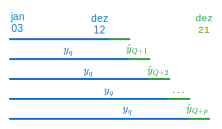
\includegraphics[width=0.7\textwidth,height=\textheight]{img/modelagem_2.png}

  }

  \caption{\label{fig-modelagem-2}Esquema de modelagem de previsões
  contínuas}

  \end{figure}%
\item
  Treino dos modelos de \emph{machine learning}: Para cada série do
  nível mais desagregado, \(y_m\), é treinado um modelo de ML com
  \(n+1\) variáveis, compostas pelas \(n\) séries --- que incluem todos
  os níveis de agregação ---, mais a própria \(y_m\) como \emph{target}
  (Tabela~\ref{tbl-modelagem}). Cada uma das \(n\) séries contam com
  \(p\) previsões obtidas no passo 1. Isso resulta em um modelo de
  reconciliação ótima para cada elemento do menor nível da hierarquia,
  combinando informações disponíveis de todos os níveis hierárquicos.
\item
  Reconciliação ótima: Com os modelos treinados, passa-se as previsões
  base obtidas na seção~\ref{sec-previsoes_base} como regressores para
  se obter as previsões reconciliadas das séries do nível mais
  desagregado \(\tilde{y}_m\).
\item
  Agregação: Assim como nos métodos analíticos de combinação ótima, a
  obtenção das previsões reconciliadas para os demais níveis de
  hierárquicos \(\tilde{y}_n\) se dá através da agregação semelhante ao
  \emph{bottom-up}, mas ao invés de se somar as previsões base
  \(\hat{y}_m\), somam-se as previsões reconciliadas \(\tilde{y}_m\).
\end{enumerate}

\begin{table}

\caption{\label{tbl-modelagem}Conjunto de dados para predição dos
modelos de ML}

\centering{

\centering
\begin{tabular}[t]{lllll}
\toprule
Target & Variável 1 & Variável 2 & ... & Variável n\\
\midrule
\cellcolor{gray!6}{$y_{1,Q+1}$} & \cellcolor{gray!6}{$\hat{y}_{1,Q+1}$} & \cellcolor{gray!6}{$\hat{y}_{2,Q+1}$} & \cellcolor{gray!6}{...} & \cellcolor{gray!6}{$\hat{y}_{n,Q+1}$}\\
$y_{2,Q+2}$ & $\hat{y}_{1,Q+2}$ & $\hat{y}_{2,Q+2}$ & ... & $\hat{y}_{n,Q+2}$\\
\cellcolor{gray!6}{...} & \cellcolor{gray!6}{...} & \cellcolor{gray!6}{...} & \cellcolor{gray!6}{...} & \cellcolor{gray!6}{...}\\
$y_{m,Q+p}$ & $\hat{y}_{1,Q+p}$ & $\hat{y}_{2,Q+p}$ & ... & $\hat{y}_{n,Q+p}$\\
\bottomrule
\end{tabular}

}

\end{table}%

Dessa forma, essa metodologia é semelhante à aplicada na reconciliação
ótima analítica, se afastando principalmente em três pontos: (i) a
utilização de algoritmos de ML ao invés de MQG, (ii) a não atribuição de
peso de forma obrigatória para todos os nós da hierarquia e (iii) no
ajuste de um modelo individual para cada série do nível mais
desagregado, permitindo maior especialização e sendo capaz de se adaptar
melhor aos diferentes padrões de cada série
(\textcite{spiliotis_hierarchical_2021}).

Um ponto negativo na metodologia proposta por
\textcite{spiliotis_hierarchical_2021} é o processo de \emph{rolling
origin} (passo 1). Esse processo requer a realização de previsões para
dentro da amostra treino, o que pode ser um problema para séries
temporais com poucas observações ou de série incompleta. No caso do
\emph{dataset} Estban, algumas das agências foram criadas após o período
escolhido para o \emph{split} em \(Q\) (dezembro/2012), sendo necessário
sua exclusão do dataset e invalidando o uso da metodologia para essas
unidades. Nesse sentido, o MinT se mostra uma opção mais viável para
aplicações no mundo real.

Nesses casos, uma alternativa para permitir o uso dos métodos de ML é
substituir o processo de \emph{rolling origin} e usar os valores
ajustados dos modelos das previsões base \(\hat{y}\) como input para os
modelos de ML. Além de permitir a inclusão de séries incompletas ---
agências criadas durante o período, no caso do \emph{dataset} Estban
---, essa abordagem também aumenta o tamanho da amostra treino em \(Q\)
observações, o que pode melhorar a performance dos modelos de ML.
Chamaremos essa estratégia de \emph{fitted base forecasts}.

Outra possibilidade de substituição do passo 1, caso as séries sejam de
tamanho suficiente, é o processo de reajuste. Esse processo consiste no
reajuste de um modelo para um novo conjunto de dados, conservando os
hiperparâmetros originais porém reestimando os coeficientes (e.g.,
treina-se um modelo autoregressivo AR(\(p\)) de coeficientes \(\phi_p\)
e então passa-se um novo conjunto de dados fora da amostra, mantendo o
hiperparâmetro \(p\) e reestimando \(\phi_p\), obtendo novos valores
ajustados). Utiliza-se então os valores reajustados para treinar os
modelos de ML. Nessa estratégia, doravante denominada de \emph{refit},
os modelos foram treinados até \(Q\) e então reajustados para \(Q+p\).
Uma restrição dessa abordagem é que, fixados os hiperparâmetros
anteriores, não necessariamente todos modelos alcançarão convergência no
reajuste de seus coeficientes para o novo conjunto de dados.

\subsection{Otimização de
hiperparâmetros}\label{otimizauxe7uxe3o-de-hiperparuxe2metros}

A maior parte dos métodos de \emph{machine learning} são altamente
parametrizáveis, sendo sua performance de generalização (para fora da
amostra) sensível à escolha de seus hiperparâmetros. Quando disponível,
os hiperparâmetros a serem otimizados e seus espaços de busca seguiram a
recomendação em \textcite{bischl_hyperparameter_2021}.

Os conjuntos de hiperparâmetros e seus intervalos são apresentados no
Apêndice \ref{apendice_hiperparametros}. Para a otimização, foram
utilizadas dois calibradores: (i) busca em grade (com resolução de 10
combinações), mais custoso em tempo de processamento, para os métodos
com menor quantidade de hiperparâmetros a serem otimizados, e (ii)
otimização bayesiana (na configuração padrão do pacote \{mlr3MBO\}),
mais eficiente para os métodos com maior quantidade de hiperparâmetros.
A estratégia de reamostragem utilizada foi a validação cruzada
\emph{k-fold} com \(k=10\).

A otimização bayesiana foi usada em todos os métodos, exceto no
\emph{elastic net}, uma vez que apenas um (no caso do \emph{lasso} e
\emph{ridge}) ou dois hiperparâmetros foram otimizados. A medida de
performance utilizada para a otimização foi a raiz do erro quadrático
médio (\emph{root mean squared error} --- RMSE).

Por fim, cada modelo foi calibrado individualmente, ou seja, cada
agência possui um conjunto de hiperparâmetros otimizados para cada um
dos 7 métodos de ML empregados para reconciliação ótima.

\section{RESULTADOS}\label{resultados}

As tabelas a seguir apresentam os resultados obtidos para o experimento.
Para fins de comparação, além do \emph{dataset} de interesse, o ESTBAN,
o experimento foi executado também para o \emph{dataset} TOURISM,
disponível no pacote \{tsibble\} \autocite{R-tsibble}, e seus resultados
reportados na seção~\ref{sec-tourism}.

As Tabela~\ref{tbl-estban-results-analiticos} e
Tabela~\ref{tbl-tourism-results-analiticos} contém as medidas de
acurácia RMSSE e MASE para os métodos analíticos de reconciliação ótima
BU (\emph{bottom-up}) e MinT, e para as previsões base, ou seja, sem
aplicar qualquer método de reconciliação. A primeira coluna especifica o
método utilizado, enquanto as demais colunas apresentam a média da
performance em cada nível de agregação.

As Tabela~\ref{tbl-estban-results-ml-rolling},
Tabela~\ref{tbl-estban-results-ml-fitted},
Tabela~\ref{tbl-estban-results-ml-refit},
Tabela~\ref{tbl-tourism-results-ml-rolling} e
Tabela~\ref{tbl-tourism-results-ml-fitted} reportam as medidas de
acurácia para os métodos de reconciliação ótima baseados em
\emph{machine learning}. Já as Tabela~\ref{tbl-estban-tempo-ml} e
Tabela~\ref{tbl-tourism-tempo-ml} reportam o tempo de processamento para
as etapas de calibragem, treino e predição desses métodos\footnote{Os
  métodos analíticos não tiveram seu tempo de processamento medidos
  porque executam quase que instantaneamente, já sinalizando uma
  vantagem para esses métodos.}.

Em geral, os métodos baseados em árvore, além de requererem maior tempo
de processamento devido a sua complexidade no espaço de hiperparâmetros,
também tenderam a perder qualidade de performance conforme suas
previsões são agregadas para formação dos níveis superiores da
hierarquia. Contrariamente, os métodos de regressão regularizada e o SVM
se mostraram mais robustos à agregação.

Nas tabelas a seguir, \textbf{negrito} indica a melhor performance entre
os métodos para aquele determinado nível de agregação, e
\underline{sublinhado} indica que aquele método de ML superou o método
analítico de melhor performance naquele nível de agregação.

\subsection{ESTBAN}\label{estban}

Nos reportes para o \emph{dataset} ESTBAN estão incluídas as médias de
performance para cada nível hierárquico e agrupado. As colunas
``agregado'', ``mesorregiao'', ``microrregiao'', ``municipio'' e
``agencia'', fazem referência à estrutura hierárquica, ou seja, tratam o
verbete de forma agregada. Já as colunas ``verbete'', ``bottom'' e
``hierarquia'', incluem também a estrutura agrupada, tratando o verbete
de forma desagregada. Detalhadamente:

\begin{itemize}
\tightlist
\item
  Agregado: performance do método para a série que representa o total,
  com os verbetes agregados, (Figura~\ref{fig-agregado}).
\item
  Mesorregião: a média das performances do método para as séries do
  agregado de cada mesorregião, com os verbetes agregados
  (Figura~\ref{fig-meso}).
\item
  Microrregião: a média das performances do método para as séries do
  agregado de cada microrregião, com os verbetes agregados
  (Figura~\ref{fig-micro}).
\item
  Município: a média das performances do método para as séries do
  agregado de cada município, com os verbetes agregados.
\item
  Agência: a média das performances do método para as séries de cada
  agência, com os verbetes agregados.
\item
  Verbete: a média das performances do método para as séries de cada
  verbete, para o total da hierarquia (Figura~\ref{fig-verbetes}).
\item
  Bottom: a média das performances do método para as séries do nível
  mais desagregado, ou seja, verbete por agência.
\item
  Hierarquia: a média das performances do método para todas as séries,
  agregadas e desagregadas.
\end{itemize}

Para o \emph{dataset} ESTBAN, não houve uma combinação de método e
estratégia que fosse consistentemente melhor ao longo de todos os níveis
de agregação. Portanto, a escolha do método e da estratégia a serem
utilizados dependerá do objetivo do pesquisador\footnote{Se o objetivo é
  a elaboração de \emph{guidance}, por exemplo, o pesquisador deve
  preferir o método e estratégia que geram as previsões mais precisas
  para o nível agregado. Já para elaboração de metas individuais, os
  níveis individuais ou regionais podem ser preferíveis.}.

Para os níveis ao topo da hierarquia, os métodos de ML se mostraram a
melhor opção para estimação. No nível agregado, o \emph{elastic net} na
estratégia \emph{refit} (Tabela~\ref{tbl-estban-results-ml-refit}) se
mostrou a melhor opção para a estimação do agregado, com 89\% de ganho
de performance sobre o MinT
(Tabela~\ref{tbl-estban-results-analiticos}), em termos de RMSSE. Da
mesma forma, para o nível de mesorregião, o \emph{elastic net} na
configuração \emph{lasso} obteve a melhor performance, performando 7\%
melhor que BU. Por outro lado, tanto nos níveis hierárquicos abaixo,
quanto nos níveis agrupados, os métodos de ML não foram capazes de
superar os métodos analíticos.

Os resultados se mostraram bastante sensíveis à estratégia utilizada. Na
métrica RMSS, nenhum método utilizando as estratégias \emph{rolling
forecast} e \emph{fitted base} foi capaz de superar o MinT em qualquer
nível de agregação, enquanto na estratégia \emph{refit} os métodos de ML
mostraram ganhos de performance com os métodos SVM e nas três
configurações do \emph{elastic net}.

Em geral, as medidas RMSSE e MASE se mostraram bastante correlacionadas,
com os métodos que obtiveram melhor performance em uma métrica também
obtendo melhor performance na outra. A exceção foi para o método
\emph{lasso} na estratégia \emph{rolling forecast}, que obteve
performance melhor que o MinT, em termos de MASE, para o nível agregado,
sendo o único resultado positivo para a estratégia \emph{rolling
forecast}.

\begin{table}

\caption{\label{tbl-estban-results-analiticos}Resultados Estban:
Acurácia dos métodos analíticos de reconciliação}

\centering{

\centering
\resizebox{\linewidth}{!}{
\begin{tabular}[t]{lrr>{}r>{}r>{}r>{}r>{}r>{}r}
\toprule
.model & agregado & mesorregiao & microrregiao & municipio & agencia & verbete & bottom & hierarquia\\
\midrule
\addlinespace[0.3em]
\multicolumn{9}{l}{\textbf{RMSSE}}\\
\cellcolor{gray!6}{\hspace{1em}base} & \cellcolor{gray!6}{0.197} & \cellcolor{gray!6}{0.690} & \cellcolor{gray!6}{0.846} & \textbf{\cellcolor{gray!6}{0.671}} & \cellcolor{gray!6}{0.717} & \cellcolor{gray!6}{0.183} & \cellcolor{gray!6}{0.656} & \cellcolor{gray!6}{0.657}\\
\hspace{1em}bu & 0.196 & 0.561 & \textbf{0.706} & 0.710 & 0.739 & 0.185 & 0.656 & 0.663\\
\cellcolor{gray!6}{\hspace{1em}mint} & \cellcolor{gray!6}{0.172} & \cellcolor{gray!6}{0.619} & \cellcolor{gray!6}{0.722} & \cellcolor{gray!6}{0.689} & \textbf{\cellcolor{gray!6}{0.712}} & \textbf{\cellcolor{gray!6}{0.140}} & \textbf{\cellcolor{gray!6}{0.634}} & \textbf{\cellcolor{gray!6}{0.641}}\\
\addlinespace[0.3em]
\multicolumn{9}{l}{\textbf{MASE}}\\
\hspace{1em}base & 0.278 & 0.818 & 0.998 & \textbf{0.790} & \textbf{0.886} & 0.250 & 0.883 & 0.847\\
\cellcolor{gray!6}{\hspace{1em}bu} & \cellcolor{gray!6}{0.240} & \cellcolor{gray!6}{0.572} & \textbf{\cellcolor{gray!6}{0.771}} & \cellcolor{gray!6}{0.820} & \cellcolor{gray!6}{0.895} & \cellcolor{gray!6}{0.221} & \textbf{\cellcolor{gray!6}{0.883}} & \cellcolor{gray!6}{0.844}\\
\hspace{1em}mint & 0.224 & 0.692 & 0.865 & 0.830 & 0.891 & \textbf{0.164} & 0.864 & \textbf{0.837}\\
\bottomrule
\end{tabular}}

}

\end{table}%

\begin{table}

\caption{\label{tbl-estban-results-ml-rolling}Resultados Estban:
Acurácia dos métodos de ML de reconciliação. Estratégia rolling
forecast.}

\centering{

\centering
\resizebox{\linewidth}{!}{
\begin{tabular}[t]{l>{}rrrrrrrr}
\toprule
modelo & agregado & mesorregiao & microrregiao & municipio & agencia & verbete & bottom & hierarquia\\
\midrule
\addlinespace[0.3em]
\multicolumn{9}{l}{\textbf{RMSSE}}\\
\cellcolor{gray!6}{\hspace{1em}elastic net} & \cellcolor{gray!6}{0.280} & \cellcolor{gray!6}{0.763} & \cellcolor{gray!6}{1.178} & \cellcolor{gray!6}{1.211} & \cellcolor{gray!6}{1.251} & \cellcolor{gray!6}{0.770} & \cellcolor{gray!6}{1.062} & \cellcolor{gray!6}{1.094}\\
\hspace{1em}lasso & 0.196 & 0.726 & 1.054 & 0.995 & 1.043 & 0.501 & 0.839 & 0.882\\
\cellcolor{gray!6}{\hspace{1em}lightgbm} & \cellcolor{gray!6}{1.407} & \cellcolor{gray!6}{1.628} & \cellcolor{gray!6}{1.530} & \cellcolor{gray!6}{1.294} & \cellcolor{gray!6}{1.322} & \cellcolor{gray!6}{0.883} & \cellcolor{gray!6}{0.972} & \cellcolor{gray!6}{1.095}\\
\hspace{1em}ranger & 1.227 & 1.397 & 1.303 & 1.118 & 1.171 & 0.725 & 0.858 & 0.949\\
\cellcolor{gray!6}{\hspace{1em}ridge} & \cellcolor{gray!6}{0.416} & \cellcolor{gray!6}{0.776} & \cellcolor{gray!6}{1.131} & \cellcolor{gray!6}{1.511} & \cellcolor{gray!6}{1.535} & \cellcolor{gray!6}{0.919} & \cellcolor{gray!6}{1.357} & \cellcolor{gray!6}{1.368}\\
\hspace{1em}svm & 0.262 & 0.745 & 0.858 & 0.853 & 0.911 & 0.234 & 0.847 & 0.838\\
\cellcolor{gray!6}{\hspace{1em}xgb} & \cellcolor{gray!6}{1.186} & \cellcolor{gray!6}{1.405} & \cellcolor{gray!6}{1.296} & \cellcolor{gray!6}{1.096} & \cellcolor{gray!6}{1.139} & \cellcolor{gray!6}{0.700} & \cellcolor{gray!6}{0.830} & \cellcolor{gray!6}{0.924}\\
\addlinespace[0.3em]
\multicolumn{9}{l}{\textbf{MASE}}\\
\hspace{1em}elastic net & 0.234 & 0.726 & 1.406 & 1.491 & 1.582 & 0.949 & 1.439 & 1.428\\
\cellcolor{gray!6}{\hspace{1em}lasso} & \underline{\cellcolor{gray!6}{0.166}} & \cellcolor{gray!6}{0.714} & \cellcolor{gray!6}{1.250} & \cellcolor{gray!6}{1.193} & \cellcolor{gray!6}{1.298} & \cellcolor{gray!6}{0.641} & \cellcolor{gray!6}{1.142} & \cellcolor{gray!6}{1.147}\\
\hspace{1em}lightgbm & 1.890 & 1.896 & 1.874 & 1.600 & 1.654 & 1.234 & 1.390 & 1.478\\
\cellcolor{gray!6}{\hspace{1em}ranger} & \cellcolor{gray!6}{1.615} & \cellcolor{gray!6}{1.560} & \cellcolor{gray!6}{1.501} & \cellcolor{gray!6}{1.332} & \cellcolor{gray!6}{1.423} & \cellcolor{gray!6}{0.996} & \cellcolor{gray!6}{1.097} & \cellcolor{gray!6}{1.177}\\
\hspace{1em}ridge & 0.402 & 0.757 & 1.315 & 1.800 & 1.881 & 1.090 & 1.790 & 1.738\\
\cellcolor{gray!6}{\hspace{1em}svm} & \cellcolor{gray!6}{0.306} & \cellcolor{gray!6}{0.684} & \cellcolor{gray!6}{0.862} & \cellcolor{gray!6}{0.991} & \cellcolor{gray!6}{1.108} & \cellcolor{gray!6}{0.290} & \cellcolor{gray!6}{1.251} & \cellcolor{gray!6}{1.143}\\
\hspace{1em}xgb & 1.542 & 1.564 & 1.479 & 1.297 & 1.373 & 0.948 & 1.022 & 1.115\\
\bottomrule
\end{tabular}}

}

\end{table}%

\begin{table}

\caption{\label{tbl-estban-results-ml-fitted}Resultados Estban: Acurácia
dos métodos de ML de reconciliação. Estratégia fitted base.}

\centering{

\centering
\resizebox{\linewidth}{!}{
\begin{tabular}[t]{lrrrrrrrr}
\toprule
modelo & agregado & mesorregiao & microrregiao & municipio & agencia & verbete & bottom & hierarquia\\
\midrule
\addlinespace[0.3em]
\multicolumn{9}{l}{\textbf{RMSSE}}\\
\cellcolor{gray!6}{\hspace{1em}elastic net} & \cellcolor{gray!6}{0.777} & \cellcolor{gray!6}{0.986} & \cellcolor{gray!6}{1.086} & \cellcolor{gray!6}{1.038} & \cellcolor{gray!6}{1.149} & \cellcolor{gray!6}{0.579} & \cellcolor{gray!6}{0.924} & \cellcolor{gray!6}{0.961}\\
\hspace{1em}lasso & 0.661 & 0.955 & 1.074 & 0.909 & 1.008 & 0.530 & 0.826 & 0.862\\
\cellcolor{gray!6}{\hspace{1em}lightgbm} & \cellcolor{gray!6}{1.495} & \cellcolor{gray!6}{1.649} & \cellcolor{gray!6}{1.557} & \cellcolor{gray!6}{1.300} & \cellcolor{gray!6}{1.342} & \cellcolor{gray!6}{0.923} & \cellcolor{gray!6}{0.999} & \cellcolor{gray!6}{1.116}\\
\hspace{1em}ranger & 1.204 & 1.397 & 1.294 & 1.098 & 1.150 & 0.694 & 0.839 & 0.930\\
\cellcolor{gray!6}{\hspace{1em}ridge} & \cellcolor{gray!6}{1.001} & \cellcolor{gray!6}{1.146} & \cellcolor{gray!6}{1.247} & \cellcolor{gray!6}{1.208} & \cellcolor{gray!6}{1.327} & \cellcolor{gray!6}{0.689} & \cellcolor{gray!6}{1.125} & \cellcolor{gray!6}{1.147}\\
\hspace{1em}svm & 0.395 & 0.929 & 0.928 & 0.934 & 0.961 & 0.319 & 0.905 & 0.898\\
\cellcolor{gray!6}{\hspace{1em}xgb} & \cellcolor{gray!6}{1.196} & \cellcolor{gray!6}{1.373} & \cellcolor{gray!6}{1.282} & \cellcolor{gray!6}{1.084} & \cellcolor{gray!6}{1.133} & \cellcolor{gray!6}{0.699} & \cellcolor{gray!6}{0.824} & \cellcolor{gray!6}{0.916}\\
\addlinespace[0.3em]
\multicolumn{9}{l}{\textbf{MASE}}\\
\hspace{1em}elastic net & 1.049 & 1.143 & 1.317 & 1.268 & 1.451 & 0.795 & 1.290 & 1.284\\
\cellcolor{gray!6}{\hspace{1em}lasso} & \cellcolor{gray!6}{0.894} & \cellcolor{gray!6}{1.087} & \cellcolor{gray!6}{1.319} & \cellcolor{gray!6}{1.114} & \cellcolor{gray!6}{1.276} & \cellcolor{gray!6}{0.728} & \cellcolor{gray!6}{1.167} & \cellcolor{gray!6}{1.162}\\
\hspace{1em}lightgbm & 2.027 & 1.931 & 1.906 & 1.610 & 1.683 & 1.302 & 1.433 & 1.512\\
\cellcolor{gray!6}{\hspace{1em}ranger} & \cellcolor{gray!6}{1.576} & \cellcolor{gray!6}{1.557} & \cellcolor{gray!6}{1.488} & \cellcolor{gray!6}{1.311} & \cellcolor{gray!6}{1.397} & \cellcolor{gray!6}{0.947} & \cellcolor{gray!6}{1.043} & \cellcolor{gray!6}{1.132}\\
\hspace{1em}ridge & 1.338 & 1.350 & 1.549 & 1.501 & 1.696 & 0.935 & 1.584 & 1.551\\
\cellcolor{gray!6}{\hspace{1em}svm} & \cellcolor{gray!6}{0.445} & \cellcolor{gray!6}{0.947} & \cellcolor{gray!6}{1.080} & \cellcolor{gray!6}{1.163} & \cellcolor{gray!6}{1.226} & \cellcolor{gray!6}{0.341} & \cellcolor{gray!6}{1.282} & \cellcolor{gray!6}{1.217}\\
\hspace{1em}xgb & 1.545 & 1.509 & 1.476 & 1.293 & 1.375 & 0.942 & 1.017 & 1.109\\
\bottomrule
\end{tabular}}

}

\end{table}%

\begin{table}

\caption{\label{tbl-estban-results-ml-refit}Resultados Estban: Acurácia
dos métodos de ML de reconciliação. Estratégia refit.}

\centering{

\centering
\resizebox{\linewidth}{!}{
\begin{tabular}[t]{l>{}r>{}rrrrrrr}
\toprule
modelo & agregado & mesorregiao & microrregiao & municipio & agencia & verbete & bottom & hierarquia\\
\midrule
\addlinespace[0.3em]
\multicolumn{9}{l}{\textbf{RMSSE}}\\
\cellcolor{gray!6}{\hspace{1em}elastic net} & \textbf{\cellcolor{gray!6}{0.090}} & \cellcolor{gray!6}{0.582} & \cellcolor{gray!6}{0.730} & \cellcolor{gray!6}{0.819} & \cellcolor{gray!6}{0.838} & \cellcolor{gray!6}{0.164} & \cellcolor{gray!6}{0.730} & \cellcolor{gray!6}{0.736}\\
\hspace{1em}lasso & \underline{0.132} & \textbf{0.523} & 0.766 & 0.757 & 0.774 & 0.187 & 0.681 & 0.693\\
\cellcolor{gray!6}{\hspace{1em}lightgbm} & \cellcolor{gray!6}{1.406} & \cellcolor{gray!6}{1.588} & \cellcolor{gray!6}{1.520} & \cellcolor{gray!6}{1.281} & \cellcolor{gray!6}{1.323} & \cellcolor{gray!6}{0.889} & \cellcolor{gray!6}{0.971} & \cellcolor{gray!6}{1.091}\\
\hspace{1em}ranger & 1.248 & 1.409 & 1.319 & 1.119 & 1.167 & 0.692 & 0.857 & 0.949\\
\cellcolor{gray!6}{\hspace{1em}ridge} & \underline{\cellcolor{gray!6}{0.141}} & \cellcolor{gray!6}{0.635} & \cellcolor{gray!6}{0.784} & \cellcolor{gray!6}{0.902} & \cellcolor{gray!6}{0.922} & \cellcolor{gray!6}{0.207} & \cellcolor{gray!6}{0.841} & \cellcolor{gray!6}{0.829}\\
\hspace{1em}svm & 0.187 & 0.743 & 0.767 & 0.792 & 0.834 & 0.295 & 0.807 & 0.792\\
\cellcolor{gray!6}{\hspace{1em}xgb} & \cellcolor{gray!6}{1.218} & \cellcolor{gray!6}{1.347} & \cellcolor{gray!6}{1.253} & \cellcolor{gray!6}{1.084} & \cellcolor{gray!6}{1.140} & \cellcolor{gray!6}{0.708} & \cellcolor{gray!6}{0.844} & \cellcolor{gray!6}{0.927}\\
\addlinespace[0.3em]
\multicolumn{9}{l}{\textbf{MASE}}\\
\hspace{1em}elastic net & \textbf{0.086} & 0.584 & 0.834 & 0.973 & 1.008 & 0.208 & 0.944 & 0.922\\
\cellcolor{gray!6}{\hspace{1em}lasso} & \underline{\cellcolor{gray!6}{0.138}} & \textbf{\cellcolor{gray!6}{0.520}} & \cellcolor{gray!6}{0.883} & \cellcolor{gray!6}{0.907} & \cellcolor{gray!6}{0.933} & \cellcolor{gray!6}{0.216} & \cellcolor{gray!6}{0.891} & \cellcolor{gray!6}{0.878}\\
\hspace{1em}lightgbm & 1.879 & 1.831 & 1.832 & 1.580 & 1.652 & 1.236 & 1.388 & 1.470\\
\cellcolor{gray!6}{\hspace{1em}ranger} & \cellcolor{gray!6}{1.636} & \cellcolor{gray!6}{1.576} & \cellcolor{gray!6}{1.526} & \cellcolor{gray!6}{1.333} & \cellcolor{gray!6}{1.418} & \cellcolor{gray!6}{0.947} & \cellcolor{gray!6}{1.065} & \cellcolor{gray!6}{1.155}\\
\hspace{1em}ridge & \underline{0.159} & 0.630 & 0.894 & 1.047 & 1.087 & 0.231 & 1.073 & 1.021\\
\cellcolor{gray!6}{\hspace{1em}svm} & \cellcolor{gray!6}{0.225} & \cellcolor{gray!6}{0.764} & \cellcolor{gray!6}{0.850} & \cellcolor{gray!6}{0.949} & \cellcolor{gray!6}{1.022} & \cellcolor{gray!6}{0.395} & \cellcolor{gray!6}{1.176} & \cellcolor{gray!6}{1.083}\\
\hspace{1em}xgb & 1.593 & 1.491 & 1.427 & 1.293 & 1.380 & 0.965 & 1.064 & 1.137\\
\bottomrule
\end{tabular}}

}

\end{table}%

\begin{table}

\caption{\label{tbl-estban-tempo-ml}Resultados Estban: Tempo de
processamento dos métodos de ML (em horas)}

\centering{

\centering
\begin{tabular}[t]{lrrrrrrr}
\toprule
  & xgb & ranger & elastic net & lasso & ridge & svm & lightgbm\\
\midrule
\cellcolor{gray!6}{refit} & \cellcolor{gray!6}{19.235} & \cellcolor{gray!6}{5.483} & \cellcolor{gray!6}{1.428} & \cellcolor{gray!6}{0.879} & \cellcolor{gray!6}{0.993} & \cellcolor{gray!6}{1.279} & \cellcolor{gray!6}{3.290}\\
fitted base & 21.758 & 5.521 & 1.363 & 0.829 & 0.924 & 1.273 & 3.341\\
\cellcolor{gray!6}{rolling forecast} & \cellcolor{gray!6}{20.908} & \cellcolor{gray!6}{5.429} & \cellcolor{gray!6}{1.345} & \cellcolor{gray!6}{0.838} & \cellcolor{gray!6}{0.929} & \cellcolor{gray!6}{1.285} & \cellcolor{gray!6}{3.377}\\
\bottomrule
\end{tabular}

}

\end{table}%

\subsection{TOURISM}\label{sec-tourism}

O \emph{dataset} TOURISM consiste na quantidade trimestral de pernoites
em visitas na Austrália entre 1998 e 2016. A estrutura é hierárquica e
agrupada, composta por 3 níveis hierárquicos --- \emph{State} (Estados),
\emph{Region} (Regiões) e total ---, e agrupado por \emph{Purpose}
(Propósito).

Assim como no \emph{dataset} ESTBAN, aqui também não houve uma
combinação de método e estratégia que fosse consistentemente melhor ao
longo de todos os níveis de agregação. Entretanto, uma tendência pode
foi observada em ambos \emph{datasets}, com os métodos de ML se
mostrando a melhor opção para estimação nos níveis ao topo da
hierarquia, enquanto os métodos analíticos se mostram melhor opção para
os níveis ao fundo da hierarquia.

\begin{table}

\caption{\label{tbl-tourism-results-analiticos}Resultados Tourism:
Acurácia dos métodos analíticos de reconciliação}

\centering{

\centering
\begin{tabular}[t]{lrrrr>{}r>{}r}
\toprule
.model & agregado & state & region & purpose & bottom & hierarquia\\
\midrule
\addlinespace[0.3em]
\multicolumn{7}{l}{\textbf{RMSSE}}\\
\cellcolor{gray!6}{\hspace{1em}base} & \cellcolor{gray!6}{1.446} & \cellcolor{gray!6}{1.260} & \cellcolor{gray!6}{1.068} & \cellcolor{gray!6}{1.265} & \cellcolor{gray!6}{0.925} & \cellcolor{gray!6}{0.976}\\
\hspace{1em}bu & 2.580 & 1.634 & 1.113 & 2.004 & 0.925 & 1.011\\
\cellcolor{gray!6}{\hspace{1em}mint} & \cellcolor{gray!6}{1.813} & \cellcolor{gray!6}{1.296} & \cellcolor{gray!6}{0.978} & \cellcolor{gray!6}{1.420} & \textbf{\cellcolor{gray!6}{0.876}} & \textbf{\cellcolor{gray!6}{0.923}}\\
\addlinespace[0.3em]
\multicolumn{7}{l}{\textbf{MASE}}\\
\hspace{1em}base & 1.533 & 1.399 & 1.132 & 1.330 & 0.979 & 1.036\\
\cellcolor{gray!6}{\hspace{1em}bu} & \cellcolor{gray!6}{3.164} & \cellcolor{gray!6}{1.877} & \cellcolor{gray!6}{1.176} & \cellcolor{gray!6}{2.323} & \cellcolor{gray!6}{0.979} & \cellcolor{gray!6}{1.078}\\
\hspace{1em}mint & 2.086 & 1.449 & 1.021 & 1.512 & \textbf{0.937} & \textbf{0.984}\\
\bottomrule
\end{tabular}

}

\end{table}%

\begin{table}

\caption{\label{tbl-tourism-results-ml-rolling}Resultados Tourism:
Acurácia dos métodos de ML de reconciliação. Estratégia rolling
forecast.}

\centering{

\centering
\begin{tabular}[t]{l>{}r>{}rr>{}rrr}
\toprule
modelo & agregado & State & Region & Purpose & bottom & hierarquia\\
\midrule
\addlinespace[0.3em]
\multicolumn{7}{l}{\textbf{RMSSE}}\\
\cellcolor{gray!6}{\hspace{1em}elastic net} & \cellcolor{gray!6}{1.990} & \cellcolor{gray!6}{1.386} & \cellcolor{gray!6}{1.086} & \cellcolor{gray!6}{1.541} & \cellcolor{gray!6}{0.988} & \cellcolor{gray!6}{1.041}\\
\hspace{1em}lasso & 1.929 & 1.373 & 1.100 & 1.523 & 1.026 & 1.069\\
\cellcolor{gray!6}{\hspace{1em}lightgbm} & \cellcolor{gray!6}{4.330} & \cellcolor{gray!6}{2.762} & \cellcolor{gray!6}{1.651} & \cellcolor{gray!6}{3.456} & \cellcolor{gray!6}{1.141} & \cellcolor{gray!6}{1.354}\\
\hspace{1em}ranger & 2.135 & 1.365 & 1.033 & 1.709 & 0.908 & 0.966\\
\cellcolor{gray!6}{\hspace{1em}ridge} & \underline{\cellcolor{gray!6}{1.256}} & \underline{\cellcolor{gray!6}{1.185}} & \cellcolor{gray!6}{1.013} & \underline{\cellcolor{gray!6}{1.202}} & \cellcolor{gray!6}{0.919} & \cellcolor{gray!6}{0.959}\\
\hspace{1em}svm & \textbf{0.940} & \textbf{1.010} & 1.076 & \textbf{1.011} & 1.100 & 1.097\\
\cellcolor{gray!6}{\hspace{1em}xgb} & \cellcolor{gray!6}{2.340} & \cellcolor{gray!6}{1.451} & \cellcolor{gray!6}{1.114} & \cellcolor{gray!6}{1.892} & \cellcolor{gray!6}{0.964} & \cellcolor{gray!6}{1.031}\\
\addlinespace[0.3em]
\multicolumn{7}{l}{\textbf{MASE}}\\
\hspace{1em}elastic net & 2.360 & 1.572 & 1.145 & 1.653 & 1.058 & 1.115\\
\cellcolor{gray!6}{\hspace{1em}lasso} & \cellcolor{gray!6}{2.264} & \cellcolor{gray!6}{1.557} & \cellcolor{gray!6}{1.168} & \cellcolor{gray!6}{1.593} & \cellcolor{gray!6}{1.110} & \cellcolor{gray!6}{1.155}\\
\hspace{1em}lightgbm & 5.505 & 3.214 & 1.763 & 4.060 & 1.200 & 1.448\\
\cellcolor{gray!6}{\hspace{1em}ranger} & \cellcolor{gray!6}{2.579} & \cellcolor{gray!6}{1.528} & \cellcolor{gray!6}{1.073} & \cellcolor{gray!6}{1.816} & \cellcolor{gray!6}{0.961} & \cellcolor{gray!6}{1.020}\\
\hspace{1em}ridge & \underline{1.343} & \underline{1.309} & 1.058 & \underline{1.192} & 0.981 & 1.020\\
\cellcolor{gray!6}{\hspace{1em}svm} & \textbf{\cellcolor{gray!6}{1.070}} & \textbf{\cellcolor{gray!6}{1.096}} & \cellcolor{gray!6}{1.140} & \textbf{\cellcolor{gray!6}{1.033}} & \cellcolor{gray!6}{1.178} & \cellcolor{gray!6}{1.174}\\
\hspace{1em}xgb & 2.888 & 1.650 & 1.162 & 2.118 & 1.013 & 1.087\\
\bottomrule
\end{tabular}

}

\end{table}%

\begin{table}

\caption{\label{tbl-tourism-results-ml-fitted}Resultados Tourism:
Acurácia dos métodos de ML de reconciliação. Estratégia fitted base.}

\centering{

\centering
\begin{tabular}[t]{lr>{}r>{}r>{}rrr}
\toprule
modelo & agregado & State & Region & Purpose & bottom & hierarquia\\
\midrule
\addlinespace[0.3em]
\multicolumn{7}{l}{\textbf{RMSSE}}\\
\cellcolor{gray!6}{\hspace{1em}elastic net} & \cellcolor{gray!6}{2.17} & \cellcolor{gray!6}{1.40} & \cellcolor{gray!6}{1.10} & \cellcolor{gray!6}{1.77} & \cellcolor{gray!6}{0.97} & \cellcolor{gray!6}{1.03}\\
\hspace{1em}lasso & 1.90 & 1.45 & 1.09 & 1.61 & 0.97 & 1.03\\
\cellcolor{gray!6}{\hspace{1em}lightgbm} & \cellcolor{gray!6}{4.33} & \cellcolor{gray!6}{2.76} & \cellcolor{gray!6}{1.65} & \cellcolor{gray!6}{3.46} & \cellcolor{gray!6}{1.14} & \cellcolor{gray!6}{1.35}\\
\hspace{1em}ranger & 2.12 & 1.36 & 1.03 & 1.72 & 0.91 & 0.96\\
\cellcolor{gray!6}{\hspace{1em}ridge} & \cellcolor{gray!6}{1.57} & \underline{\cellcolor{gray!6}{1.16}} & \textbf{\cellcolor{gray!6}{0.97}} & \cellcolor{gray!6}{1.29} & \cellcolor{gray!6}{0.90} & \cellcolor{gray!6}{0.93}\\
\hspace{1em}svm & 1.50 & \underline{1.19} & 1.05 & 1.38 & 1.04 & 1.05\\
\cellcolor{gray!6}{\hspace{1em}xgb} & \cellcolor{gray!6}{2.27} & \cellcolor{gray!6}{1.42} & \cellcolor{gray!6}{1.10} & \cellcolor{gray!6}{1.83} & \cellcolor{gray!6}{0.96} & \cellcolor{gray!6}{1.02}\\
\addlinespace[0.3em]
\multicolumn{7}{l}{\textbf{MASE}}\\
\hspace{1em}elastic net & 2.59 & 1.57 & 1.16 & 1.95 & 1.04 & 1.10\\
\cellcolor{gray!6}{\hspace{1em}lasso} & \cellcolor{gray!6}{2.21} & \cellcolor{gray!6}{1.67} & \cellcolor{gray!6}{1.16} & \cellcolor{gray!6}{1.73} & \cellcolor{gray!6}{1.04} & \cellcolor{gray!6}{1.11}\\
\hspace{1em}lightgbm & 5.50 & 3.21 & 1.76 & 4.06 & 1.20 & 1.45\\
\cellcolor{gray!6}{\hspace{1em}ranger} & \cellcolor{gray!6}{2.54} & \cellcolor{gray!6}{1.54} & \cellcolor{gray!6}{1.07} & \cellcolor{gray!6}{1.84} & \cellcolor{gray!6}{0.97} & \cellcolor{gray!6}{1.02}\\
\hspace{1em}ridge & 1.77 & \underline{1.29} & \textbf{1.01} & \underline{1.31} & 0.96 & 0.99\\
\cellcolor{gray!6}{\hspace{1em}svm} & \cellcolor{gray!6}{1.75} & \underline{\cellcolor{gray!6}{1.30}} & \cellcolor{gray!6}{1.09} & \cellcolor{gray!6}{1.36} & \cellcolor{gray!6}{1.10} & \cellcolor{gray!6}{1.11}\\
\hspace{1em}xgb & 2.79 & 1.62 & 1.15 & 2.04 & 1.01 & 1.08\\
\bottomrule
\end{tabular}

}

\end{table}%

\begin{table}

\caption{\label{tbl-tourism-results-ml-refit}Resultados Tourism:
Acurácia dos métodos de ML de reconciliação. Estratégia refit.}

\centering{

\centering
\begin{tabular}[t]{lrrrrrr}
\toprule
modelo & agregado & State & Region & Purpose & bottom & hierarquia\\
\midrule
\addlinespace[0.3em]
\multicolumn{7}{l}{\textbf{RMSSE}}\\
\cellcolor{gray!6}{\hspace{1em}lightgbm} & \cellcolor{gray!6}{4.33} & \cellcolor{gray!6}{2.76} & \cellcolor{gray!6}{1.65} & \cellcolor{gray!6}{3.46} & \cellcolor{gray!6}{1.14} & \cellcolor{gray!6}{1.35}\\
\hspace{1em}ranger & 2.58 & 1.55 & 1.11 & 2.01 & 0.92 & 1.01\\
\cellcolor{gray!6}{\hspace{1em}xgb} & \cellcolor{gray!6}{3.14} & \cellcolor{gray!6}{1.93} & \cellcolor{gray!6}{1.28} & \cellcolor{gray!6}{2.44} & \cellcolor{gray!6}{1.02} & \cellcolor{gray!6}{1.14}\\
\addlinespace[0.3em]
\multicolumn{7}{l}{\textbf{MASE}}\\
\hspace{1em}lightgbm & 5.50 & 3.21 & 1.76 & 4.06 & 1.20 & 1.45\\
\cellcolor{gray!6}{\hspace{1em}ranger} & \cellcolor{gray!6}{3.18} & \cellcolor{gray!6}{1.76} & \cellcolor{gray!6}{1.17} & \cellcolor{gray!6}{2.24} & \cellcolor{gray!6}{0.98} & \cellcolor{gray!6}{1.07}\\
\hspace{1em}xgb & 3.93 & 2.27 & 1.38 & 2.86 & 1.07 & 1.21\\
\bottomrule
\end{tabular}

}

\end{table}%

\begin{table}

\caption{\label{tbl-tourism-tempo-ml}Resultados Tourism: Tempo de
processamento dos métodos de ML (em horas)}

\centering{

\centering
\begin{tabular}[t]{lrrrrrrr}
\toprule
  & xgb & ranger & elastic net & lasso & ridge & svm & lightgbm\\
\midrule
\cellcolor{gray!6}{fitted base} & \cellcolor{gray!6}{15.767} & \cellcolor{gray!6}{3.687} & \cellcolor{gray!6}{1.540} & \cellcolor{gray!6}{1.282} & \cellcolor{gray!6}{1.371} & \cellcolor{gray!6}{1.977} & \cellcolor{gray!6}{3.535}\\
rolling forecast & 12.087 & 2.987 & 0.957 & 0.796 & 1.073 & 2.035 & 3.596\\
\cellcolor{gray!6}{refit} & \cellcolor{gray!6}{24.627} & \cellcolor{gray!6}{15.386} & \cellcolor{gray!6}{6.006} & \cellcolor{gray!6}{4.968} & \cellcolor{gray!6}{5.323} & \cellcolor{gray!6}{10.474} & \cellcolor{gray!6}{19.362}\\
\bottomrule
\end{tabular}

}

\end{table}%

\section{CONCLUSÃO}\label{conclusuxe3o}

Neste trabalho, foram apresentados experimentos de reconciliação ótima
para séries temporais hierárquicas e agrupadas, utilizando métodos
analíticos e de \emph{machine learning} com o objetivo de obter
coerência e ganhos de acurácia nas previsões de saldos de empréstimos e
financiamentos do Banco do Estado do Espírito Santo. Pesquisas
anteriores já haviam mostrado que a reconciliação ótima pode trazer
ganhos de acurácia, e que métodos de \emph{machine learning} podem ser
competitivos em relação aos métodos analíticos.

Este trabalho trouxe, além dos métodos de floresta aleatória e
\emph{gradient boosting} já trabalhados em
\textcite{spiliotis_hierarchical_2021}, o método de regressão
regularizada \emph{elastic net} e o \emph{support vector machines}, além
de avaliar outro método de \emph{gradient boosting}, o \emph{lightGBM}.
Paralelamente, este trabalho propôs duas estratégias alternativas para a
metodologia de reconciliação ótima baseada em \emph{machine learning}
proposta originalmente em \textcite{spiliotis_hierarchical_2021}.

Os resultados obtidos para o \emph{dataset} ESTBAN mostraram,
primeiramente, que não houve uma combinação de método e estratégia que
obtivesse melhor performance de maneira consistente ao longo de todos os
níveis hierárquicos. Dessa forma, a escolha do método e da estratégia a
serem utilizados dependerá do objetivo do pesquisador. Para os níveis ao
topo da hierarquia, a combinação correta de método e estratégia de
estimação (\emph{elastic net} + \emph{refit}) gerou até 89\% de ganho de
performance no nível mais agregado, permitindo à instituição financeira
maior precisão para tomada de decisão e planejamento estratégico, além
de sinalizar maior confiança nas estimativas comunicadas ao mercado e
aos investidores. Por outro lado, para os níveis inferiores na estrutura
hierárquica, os métodos analíticos se mostraram a melhor escolha. Isso
sugere que, com o objetivo de elaboração de metas individuais --- seja
para as agências ou superintendências regionais ---, os métodos
analíticos ainda são preferíveis.

Os restultados para o \emph{dataset} ESTBAN também mostram que o
resultado da reconciliação ótima é sensível à estratégia utilizada.
Apenas na estratégia \emph{refit} que os ganhos de performance foram
observados, enquanto nas estratégias \emph{rolling forecast} e
\emph{fitted base} os métodos de ML não foram capazes de superar os
métodos analíticos.

O mesmo padrão em relação à performance ao logo dos níveis de agregação
pôde ser observado no \emph{dataset} TOURISM. Foi possível encontrar uma
combinação de método de ML e estratégia capaz de superar os métodos
analíticos para os níveis mais agregados, mas não para os níveis mais
desagregados. Nesse \emph{dataset}, os métodos de ML superaram os
analíticos em todos os níveis de agregação, exceto no mais desagregado,
com os métodos \emph{support vector machines} e \emph{elastic net}
liderando a performance tanto nas estratégias \emph{rolling forecast}
quanto \emph{fitted base}.

Contrariamente aos resultados de \textcite{spiliotis_hierarchical_2021},
em ambos \emph{datasets}, os métodos de ML baseados em árvore de decisão
(\emph{XGBoost}, \emph{ranger} e \emph{lightGBM}) não foram capazes de
superar os métodos analíticos em nenhum nível de agregação.

Para pesquisas futuras, pode-se investigar se a performance dos
diferentes métodos e estratégias estão relacionadas às características
das séries temporais, por exemplo:

\begin{itemize}
\tightlist
\item
  Os efeitos do ruído de previsão: se os diferentes métodos e
  estratégias exibem aumento ou deterioração de performance quando as
  previsões individuais são mais ou menos ruidosas (i.e.~se a variância
  do erro das previsões individuais é maior ou menor).
\item
  Os efeitos de correlação entre as séries: se os métodos e estratégias
  exibem aumento ou deterioração de performance quando as séries
  temporais no menor nível hierárquico são mais ou menos
  correlacionadas.
\item
  Os efeitos de componentes sazonais: se os métodos e estratégias exibem
  aumento ou deterioração de performance quando as séries temporais do
  menor nível hierárquico possuem ou não componentes sazonais.
\item
  Os efeitos do tamanho da hierarquia: verificar se os métodos e
  estratégias exibem aumento ou deterioração de performance quando a
  hierarquia é mais ou menos profunda (i.e.~possui mais ou menos níveis
  hierárquicos).
\end{itemize}


\printbibliography[title=REFERÊNCIAS]


% elementos pós-textuais 
\postextual

% apêndice 
\begin{apendicesenv}
\partapendices

% Apêndice A
\chapter{MÉTODOS DE RECONCILIAÇÃO ÓTIMA}\label{apendice_metodos_reconciliacao}

\section{Métodos analíticos de reconciliação
ótima}\label{muxe9todos-analuxedticos-de-reconciliauxe7uxe3o-uxf3tima}

Os métodos analíticos de reconciliação ótima são aqueles que estimam a
matriz de reconciliação, \(\mathbfit{G}\), através de regressão linear.
Isso resulta na redefinição das previsões do nível mais desagregado como
uma combinação linear\footnote{Por essa razão, esses métodos são também
  chamados de métodos de combinação.} das previsões de todos os
elementos de todos os níveis da hierarquia, utilizando, assim, toda a
informação disponível.

O estado-da-arte para esse tipo de método é o \emph{MinT}
\autocite{wickramasuriya_optimal_2019}. Nele, o objetivo é minimizar o
erro das previsões reconciliadas:

\begin{equation}\phantomsection\label{eq-mint1}{
\mathbfit{\tilde{e}}_{t+h|t} = \mathbfit{y}_{t+h} - \mathbfit{\tilde{y}}_{t+h|t}
}\end{equation}

Essa equação pode ser reescrita como
\(\mathbfit{\tilde{e}}_t = \mathbfit{SG\hat{e}}_t\), que tem variância
dada por\footnote{Ver demonstração \ref{proposicao3}.}

\begin{equation}\phantomsection\label{eq-mint2}{
\text{Var}[\mathbfit{\tilde{e}}] = \mathbfit{SG\hat{W}}_{t+h|t}\mathbfit{G'S'}
}\end{equation}

\noindent em que \(\mathbfit{\hat{W}}_{t+h|t}\) é a matriz de
variância-covariância dos erros de previsão base.

A abordagem consiste então em se obter um valor de \(\mathbfit{G}\) que
minimize o traço de
\(\text{Var}[\mathbfit{y}_{t+h} - \mathbfit{\tilde{y}}_{t+h|t}]\). Isso
resultaria no melhor (variância mínima) estimador linear não
viesado\footnote{A ausência de viés é garantida pela
  \nameref{proposicao1}.} \autocite{wickramasuriya_optimal_2019}.

\begin{equation}\phantomsection\label{eq-mint3}{
\mathbfit{G} = (\mathbfit{S'\hat{W}}^\dagger_{t+h|t}\mathbfit{S})^{-1}\mathbfit{S'\hat{W}}^\dagger_{t+h|t}
}\end{equation}

\noindent em que \(\mathbfit{\hat{W}}^\dagger_{t+h|t}\) é a inversa
generalizada de Moore-Penrose para
\(\mathbfit{\hat{W}}_{t+h|t}\)\footnote{A necessidade da inversa
  generalizada aqui é trivial, uma vez que a inversa regular, do tipo
  \(\mathbfit{A}^{-1}\), requer matriz quadrada, o que não acontece no
  caso de séries temporais hierárquicas, uma vez que, necessariamente,
  tem-se \(n>m\) (\(n=m+\text{número de nós de agregação}\)). Além
  disso, \(\mathbfit{\hat{W}}\) é posto incompleto (ver demonstração
  \ref{proposicao4}).}. Essa formulação corresponde a um problema de
regressão por mínimos quadradados generalizados, considerando
\(\mathbfit{S}\) como a matriz de preditores e \(\mathbfit{G}\) os
coeficientes a serem estimados. Consequentemente, as previsões ótimas
reconciliadas são dadas por

\begin{equation}\phantomsection\label{eq-mint4}{
\mathbfit{\tilde{y}}_{t+h|t} = \mathbfit{S}(\mathbfit{S'\hat{W}}^\dagger_{t+h|t}\mathbfit{S})^{-1}\mathbfit{S'\hat{W}}^\dagger_{t+h|t}\mathbfit{\hat{y}}_{t+h|t}
}\end{equation}

\section{Métodos de reconciliação ótima baseados em aprendizado de
máquina}\label{muxe9todos-de-reconciliauxe7uxe3o-uxf3tima-baseados-em-aprendizado-de-muxe1quina}

Embora os métodos de ML também sejam utilizados no contexto de previsão
de séries temporais, é importante ressaltar que este não é caso. As
previsões de séries temporais são realizadas anteriormente, na obtenção
das previsões base \(\hat{y}_t\). Nada impede que essas previsões sejam
obtidas por um modelo de ML, mas isso não é o foco deste trabalho.

A aplicação dos métodos de ML aqui ocorrem na reconciliação, ou seja, na
combinação contemporânea, \emph{cross section}, das previsões base que,
por sua vez, podem ter sido obtidas através de qualquer método.

\subsection{Elastic Net}\label{elastic-net}

O \emph{elastic net} \autocite{zou_regularization_2005} é um método de
regressão regularizada que combina as normas \(L_1\) e \(L_2\), as
penalidades do \emph{lasso} e do \emph{ridge}, respectivamente. A função
objetivo a ser minimizada é dada por

\begin{equation}\phantomsection\label{eq-elastic_net}{
L(\lambda_1, \lambda_2, \mathbfit{\beta}) = |\mathbf{y} - \mathbf{X}\mathbfit{\beta}|^2 + \lambda_2|\mathbfit{\beta}|^2 + \lambda_1|\mathbfit{\beta}|_1
}\end{equation}

\noindent em que \(\lambda_1\) e \(\lambda_2\) são os parâmetros de
regularização e \(\mathbfit{\beta}\) é o vetor de coeficientes a serem
estimados. A solução para essa função objetivo é dada por\footnote{Sob o
  valor otimizado ainda é aplicada correção de escala na forma
  \((1+\lambda_2)\mathbfit{\hat{\beta}}\). Ver
  \textcite{zou_regularization_2005}.}

\begin{equation}\phantomsection\label{eq-elastic_net_solution}{
\mathbfit{\hat{\beta}} = \arg \min_{\mathbfit{\beta}} |\mathbf{y}-\mathbf{X}\mathbfit{\beta}|^2 \text{, sujeito a } (1-\alpha)|\mathbfit{\beta}|_1 + \alpha|\mathbfit{\beta}|^2 \leq t
}\end{equation}

\noindent com \(\alpha = \frac{\lambda_2}{\lambda_1 + \lambda_2}\) e
\(t \in \mathbb{R}^+\).

A função \((1-\alpha)|\mathbfit{\beta}|_1 + \alpha|\mathbfit{\beta}|^2\)
é a penalidade \emph{elastic net}, uma combinação das penalidades
\emph{lasso} e \emph{ridge}. O parâmetro \(\alpha\) controla a mistura
das duas penalidades, incluindo os casos extremos. Note que
\(\alpha = 0 \implies \lambda_2 = 0\), resultando em uma penalidade
exclusivamente \emph{lasso}, enquanto
\(\alpha = 1 \implies \lambda_1 = 0\), e a penalidade é apenas do tipo
\emph{ridge}.

Portanto o \emph{elastic net} é um método de \emph{shrinkage}, uma vez
que a penalidade \emph{ridge} reduz o tamanho dos coeficientes, e de
\emph{seleção de variáveis}, uma vez que a penalidade \emph{lasso} tende
a anular os coeficientes de variáveis irrelevantes. Essas propriedades
são desejáveis para a reconciliação de séries temporais, uma vez que a
estrutura hierárquica pode conter séries insignificantes para a previsão
de outras séries.

Diferentemente dos métodos analíticos estudados, o \emph{elastic net}
não possui uma solução fechada. Portanto, é necessário utilizar métodos
iterativos para encontrar o valor ótimo de \(\mathbfit{\hat{\beta}}\) e
\textcite{zou_regularization_2005} utilizam validação cruzada \(k\)-fold
para encontrar quais os valores de \(\lambda_1\) e \(\lambda_2\) que
minimizam o resíduo. Nesse sentido, dado a metodologia de processo
iterativo envolvendo calibragem de hiperparâmetros e reamostragem,
podemos classificar o \emph{elastic net} como um método de \emph{machine
learning}.

\subsection{Gradient Boosting}\label{gradient-boosting}

Como cada uma das diversas implementações de \emph{gradient boosting}
possui sua teoria adjacente, e não é de objetivo deste trabalho detalhar
o funcionamento de cada uma delas, trabalharemos apenas sua intuição.

Assim como os métodos de floresta aleatória, os métodos de
\emph{gradient boosting} também são métodos de conjuntos de árvores. A
diferença se dá na forma como os modelos são treinados. \emph{Gradient
boosting} são métodos que combinam as predições de vários modelos fracos
parar formar um conjunto --- \emph{ensemble}, na definição mais usual,
ou comitê (\emph{committee}), na definição de
\textcite{hastie_elements_2009} quando usado para classificação --- mais
complexo e preciso (forte).

Um estimador fraco é aquele que tem desempenho apenas ligeiramente
melhor que o acaso. O propósito do \emph{boosting} é produzir uma
sequencia de estimadores fracos, cada um deles focado nos erros dos
estimadores anteriores. A cada iteração, as observações classificadas
incorretamente (no caso de uma tarefa de classificação) ou de maior
variância (no caso de uma tarefa de regressão) na iteração anterior têm
seu peso aumentado, e vice-versa. Dessa forma, o modelo subsequente
formado na próxima iteração é obrigado a se concentrar nas observações
onde as iterações anteriores falharam. Isso que significa transformar um
conjunto de estimadores fracos em um conjunto forte.

O \emph{gradient boosting} é uma extensão do \emph{boosting} que utiliza
o gradiente da função de perda como critério de otimização, de forma que
esta se dá na direção em que a função de perda decresce mais rapidamente
a cada iteração. Os métodos utilizados neste trabalho são o
\emph{XGBoost} \autocite{chen_xgboost_2016} e o \emph{LightGBM}
\autocite{ke_lightgbm_2017}.

Um das principais diferenças entre os dois métodos é a forma como as
árvores são construídas. O \emph{XGBoost} cresce suas árvores de forma
\emph{level-wise}, ou seja, cresce todas as folhas do último nível de
uma árvore de uma vez, adicionando mais um nível de profundidade
completo a cada iteração (Figura~\ref{fig-xgboost}). Já o
\emph{LightGBM} cresce suas árvores de forma \emph{leaf-wise}, ou seja,
cresce uma folha por vez, aprofundando a árvore apenas no nó que resulta
na maior variação negativa na função de perda
(Figura~\ref{fig-lightgbm}).

\begin{figure}

\begin{minipage}{\linewidth}

\centering{

\includegraphics[width=0.7\textwidth,height=\textheight]{img/xgboost.png}

}

\subcaption{\label{fig-xgboost}\emph{level-wise}}

\end{minipage}%
\newline
\begin{minipage}{\linewidth}

\centering{

\includegraphics[width=0.7\textwidth,height=\textheight]{img/lightgbm.png}

}

\subcaption{\label{fig-lightgbm}\emph{leaf-wise}}

\end{minipage}%

\caption{\label{fig-tree-growth}Crescimento de árvores em algoritmos de
\emph{boosting}.}

\end{figure}%

\subsection{Random Forest}\label{random-forest}

Floresta aleatória é um método de aprendizado de máquina que utiliza
conjuntos de árvores de decisão descorrelatadas\footnote{As árvores de
  decisão são descorrelatadas no sentido que, ao contrário os métodos de
  \emph{boosting trees}, a próxima árvore não é construída com base na
  iteração anterior (processo de fortalecimento).} para classificação ou
regressão. O método consiste em treinar várias árvores de decisão em
subconjuntos aleatórios dos dados de treinamento e, então, combinar suas
predições \autocite{hastie_elements_2009}. A aleatoriedade é introduzida
de duas formas: na seleção das observações e na seleção das variáveis
preditoras.

A intuição para seu algoritmo para regressão é simples e a ideia geral
é, para cada árvore de decisão, particionar recursivamente nós de
tamanho \(N\) em dois nós filhos de forma a aumentar a complexidade do
modelo e minimizar a função de custo. Se a próxima partição de um nó
resultar em um ou ambos nós filhos de tamanho menor que um mínimo
estabelecido via hiperparâmetro, a partição é interrompida (Algoritmo
\ref{alg-rf}).

\begin{algorithm}
\caption{Floresta aleatória para regressão}\label{alg-rf}

${T_1, T_2, ..., T_b}$ é uma floresta aleatória de $B$ árvores de decisão. \\
\BlankLine
$i \in \mathbb{N}$ é a quantidade de observações em um nó. \\
\BlankLine
$n_{min} \in \mathbb{N}$ é o número mínimo de observações em um nó. \\
\BlankLine
\For{$b = 1 \to B$}{
  1. Toma uma amostra de tamanho $N$ dos dados de treino. \\
  \While{$i < n_{min}$} {
    a. Seleciona $j$ variáveis aleatoriamente. \\
    b. Escolhe a melhor variável para \textit{split} dentre $j$. \\
    c. Divide o nó em dois nós filhos. \\
    \If{Nenhum dos nós filhos tem $i < n_{min}$} {
      d. Repete os passos a-c para cada nó filho.
    }
  }
}
\BlankLine
2. Produz um conjunto de árvores $\{T_b\}_1^B$.
\BlankLine
3. Realiza a predição para cada árvore $T_b$ em um ponto $x$ e calcula a média das predições:
$$\hat{f}(x) = \frac{1}{B}\sum_{b=1}^B T_b(x)$$

\end{algorithm}

\subsection{Support Vector Machines}\label{support-vector-machines}

A intuição do métodos de SVMs é mais facilmente compreendida a partir de
uma tarefa de classificação de duas classes. Nesse caso, o objetivo é
encontrar um hiperplano (i.e.~um sub-espaço de dimensão \(n-1\)) que
separe as classes de forma que a margem entre o hiperplano e os pontos
de cada classe seja a maior possível. Então, dado um conjunto de \(N\)
pares de observações e suas respectivas classes,
\(\{(x_i, y_i)\}_{i=1}^N\), em que \(x_i \in \mathbb{R}^p\) e
\(y_i \in \{-1, 1\}\), queremos encontrar o hiperplano definido por

\[
\{x: f(x) = x^T\beta + \beta_0 = 0\}
\]

\noindent sendo \(f(x)\) a distância ortogonal entre \(x\) e o
hiperplano \(f(x) = x^T\beta + \beta_0 = 0\), e \(M\) a margem entre as
classes, definida como a distância ortogonal entre os pontos mais
próximos de cada classe e o hiperplano \autocite{hastie_elements_2009}.
Portanto, o problema de otimização é dado por

\begin{equation}\phantomsection\label{eq-svm}{
\begin{aligned}
& \underset{\beta, \beta_0}{\text{max}}
& & M \\
& \text{sujeito a}
& & y_i(x_i^T\beta + \beta_0) \geq M, \quad i = 1, ..., N
\end{aligned}
}\end{equation}

Quando pode-se encontrar um hiperplano com
\(y_if(x_i) > 0 \quad \forall i\), tem-se o caso da construção de uma
solução única para um hiperplano entre duas classes perfeitamente
separadas pela maior margem possível (Figura~\ref{fig-svm1}).

\begin{figure}

\begin{minipage}{\linewidth}

\centering{

\includegraphics[width=0.4\textwidth,height=\textheight]{img/svm1.png}

}

\subcaption{\label{fig-svm1}Hiperplano entre duas classes perfeitamente
separáveis.}

\end{minipage}%
\newline
\begin{minipage}{\linewidth}

\centering{

\includegraphics[width=0.4\textwidth,height=\textheight]{img/svm2.png}

}

\subcaption{\label{fig-svm2}Hiperplano entre duas classes não
separáveis.}

\end{minipage}%

\caption{\label{fig-svm}\emph{Support vector classifiers}. Fonte:
\textcite{hastie_elements_2009}.}

\end{figure}%

Entretanto, no mundo real, dificilmente um problema de classificação
será linearmente separável. Paara contornar esse obstáculo, é possível
introduzir variáveis de folga \(\xi_i \geq 0\) para cada observação
(Figura~\ref{fig-svm2}), de forma que a restrição se torne

\begin{equation}\phantomsection\label{eq-svm2}{
y_i(x_i^T\beta + \beta_0) \geq M(1 - \xi_i), \quad i = 1, ..., N
}\end{equation}

\noindent e a função objetivo se torne

\begin{equation}\phantomsection\label{eq-svm3}{
\min{||\beta||} \quad \text{sujeito a}
\left\{
  \begin{aligned}
    &\quad y_i(x_i^T\beta + \beta_0) \geq M(1 - \xi_i) \quad \forall i, \\
    &\quad \xi_i \geq 0, \sum{\xi_i} \leq \text{constante}
  \end{aligned}
\right\}
}\end{equation}

Para estender essa ideia para problemas de regressão, é necessário
introduzir uma função de perda \(\epsilon\)-insensível, que penaliza
apenas os erros maiores que \(\epsilon\), de forma que os erros menores
são ignorados durante a otimização, assim como as observações
localizadas no lado correto do hiperplano são ignoradas no problema de
classificação. A função objetivo se torna

\begin{equation}\phantomsection\label{eq-svm4}{
\min{||\beta||} \quad \text{sujeito a}
\left\{
  \begin{aligned}
    &\quad |y_i - x_i^T\beta - \beta_0| \leq \epsilon \quad \forall i, \\
    &\quad \sum{|\beta_j|} \leq \text{constante}
  \end{aligned}
\right\}
}\end{equation}

\chapter{DEMONSTRAÇÕES} \label{apendice_demonstracoes}

% proposição 1
\begin{proposition}[condição de ausência de viés em $\mathbfit{\tilde{y}}$]
  \label{proposicao1}

  Se as previsões reconciliadas são não viesadas, então $\mathbfit{SGS=S}$, ou seja, $\mathbfit{G}$ é inversa generalizada de $\mathbfit{S}$.

\end{proposition}

\begin{proof}
  \begin{equation} \label{eq:ap1}
    \mathbfit{\tilde{y}}_{t+h|t} = \mathbfit{SG\hat{y}}_{t+h|t} 
  \end{equation}

  Se $\mathbfit{\hat{y}}_{t+h|t}$ é não viesado, então 

  \begin{equation} \label{eq:ap2}
      \mathbb{E}[\mathbfit{\hat{y}}_{t+h|t}] = \mathbb{E}[\mathbfit{y}_{t+h|t}] = \mathbfit{Sb}_t
  \end{equation}

  Da mesma forma, se espera-se que as previsões reconciliadas não sejam viesadas,
  \begin{equation} \label{eq:ap3}
      \mathbb{E}[\mathbfit{\tilde{y}}_{t+h|t}] = \mathbb{E}[\mathbfit{y}_{t+h|t}] = \mathbfit{Sb}_t
  \end{equation}

  Substituindo \eqref{eq:ap2} em \eqref{eq:ap1}, temos

  \begin{equation} \label{eq:ap4}
      \mathbfit{\tilde{y}}_{t+h|t} = \mathbfit{SGSb}_t 
  \end{equation}

  Logo, para manter a igualdade entre \eqref{eq:ap1} e \eqref{eq:ap4}, $\mathbfit{SGS=S}$

\end{proof}

% proposição 2
\begin{proposition}
  \label{proposicao2}

  $\mathbfit{\tilde{e}}_t = \mathbfit{SG\hat{e}}_t$.

\end{proposition}

\begin{proof}
  \begin{equation} \label{eq:apa22}
    \mathbfit{\tilde{e}}_{t+h|t} = \mathbfit{y}_{t+h} - \mathbfit{\tilde{y}}_{t +h|t}
  \end{equation}

  Substituindo \eqref{eq:ap1} em \eqref{eq:apa22},

  \begin{align} \label{eq:apa23}
    \mathbfit{\tilde{e}}_{t+h|t} &= \mathbfit{y}_{t+h} - \mathbfit{SG\hat{y}}_{t+h|t}
  \end{align}

  Lembrando que, por definição, $\mathbfit{y}_{t+h} = \mathbfit{\hat{y}}_{t+h|t} + \mathbfit{\hat{e}}_{t+h|t}$, então

  \begin{align} \label{eq:apa24}
    \mathbfit{\tilde{e}}_{t+h|t} &= \mathbfit{\hat{y}}_{t+h|t} + \mathbfit{\hat {e}}_{t+h|t} - \mathbfit{SG\hat{y}}_{t+h|t} \\
    &= \mathbfit{\hat{e}}_{t+h|t} + \mathbfit{\hat{y}}_{t+h|t}(\mathbfit{I-SG)}
  \end{align}

  Usando a definição novamente, temos que

  \begin{align}
    \mathbfit{\tilde{e}}_{t+h|t} &= \mathbfit{\hat{e}}_{t+h|t} + (\mathbfit{y}_ {t+h} - \mathbfit{\hat{e}}_{t+h|t})(\mathbfit{I-SG)} \\
    &= \mathbfit{y}_{t+h} - \mathbfit{SGy}_{t+h|t} + \mathbfit{SG\hat{e}}_{t+h| t} \\
    &=  \mathbfit{y}_{t+h}(\mathbfit{I-SG}) + \mathbfit{SG\hat{e}}_{t+h|t}  \label{eq:apa25}
  \end{align}

  Substituindo \eqref{eq-vetor_b} em \eqref{eq:apa25}, temos

  \begin{align}
    \mathbfit{\tilde{e}}_{t+h|t} &=  \mathbfit{Sb}_{t+h}(\mathbfit{I-SG}) +  \mathbfit{SG\hat{e}}_{t+h|t} \\
    &=  \mathbfit{Sb}_{t+h} - \mathbfit{Sb}_{t+h}\mathbfit{SG} + \mathbfit {SG\hat{e}}_{t+h|t}  \\
    &=  \mathbfit{Sb}_{t+h} - \mathbfit{(G'S')(b'}_{t+h}\mathbfit{S')} +   \mathbfit{SG\hat{e}}_{t+h|t}  \\
    &=  \mathbfit{Sb}_{t+h} - \mathbfit{SG}\mathbfit{Sb}_{t+h} + \mathbfit {SG\hat{e}}_{t+h|t}
  \end{align}

  Finalmente, pela \nameref{proposicao1}, temos que

  \begin{align}
    \mathbfit{\tilde{e}}_{t+h|t} &=  \mathbfit{Sb}_{t+h} - \mathbfit{Sb}_{t+h}  + \mathbfit{SG\hat{e}}_{t+h|t}  \\
    &= \mathbfit{SG\hat{e}}_{t+h|t}
  \end{align}
\end{proof}

% proposição 3
\begin{proposition}
  \label{proposicao3}

  $\text{Var}[\mathbfit{\tilde{e}}_t] = \mathbfit{SG\hat{W}G'S'}$.

\end{proposition}

\begin{proof}
  Por \ref{proposicao2}, temos que

  \begin{align}
    \text{Var}[\mathbfit{\tilde{e}}] &= \mathbb{E}[\mathbfit{(SG\hat{e})(SG\hat {e})'}] \\
    &= \mathbb{E}[\mathbfit{SG\hat{e}\hat{e}'G'S'}] \\
    &= \mathbfit{SG\hat{W}G'S'}
  \end{align}

  Em que $\mathbfit{\hat{W}}$ é a matriz de variância-covariância dos erros de  previsão base.
\end{proof}

% proposição 4
\begin{proposition}
  \label{proposicao4}

  $\mathbfit{\hat{W}}$ é posto incompleto.

\end{proposition}

\begin{proof}
  Pela propriedade do vínculo do posto do produto de matrizes, ou seja, $pos(\mathbfit{AB}) \leq min(pos(\mathbfit{A}), pos(\mathbfit{B}))$, temos que
  
  \begin{equation}
    pos(\mathbfit{SG\hat{e}}_{t+h|t}) \leq min(pos(\mathbfit{S}), pos(\mathbfit{G}), pos(\mathbfit{\hat{e}}_{t+h|t})) \label{eq:ap_a_4_1}
  \end{equation}

  Como $\mathbfit{S}$ é a representação matricial de uma estrutura hierárquica, em que os nós pais totalizam os nós filhos, $\mathbfit{S}$ apresenta, por hipótese, dependência linear e, consequentemente, posto incompleto.

  Pela equação \eqref{eq:ap_a_4_1}, segue que $\mathbfit{\tilde{e}}$ é posto incompleto. Da mesma forma, $pos(\mathbfit{\tilde{e}\tilde{e}'}) \leq min(pos(\mathbfit{\tilde{e}}), pos(\mathbfit{\tilde{e}'}))$. Portanto, $\mathbfit{\hat{W}}$ é posto incompleto.
\end{proof}

% apêndice B
\chapter{CONJUNTO DE HIPERPARÂMETROS} \label{apendice_hiperparametros}

\begin{table}

  \caption{\label{tab:tbl-hip-xgboost}Intervalos de hiperparâmetros para \{xgboost\}}
  \centering
  \begin{tabular}[t]{llll}
  \toprule
  Hiperparâmetro & Descrição & Intervalo & Trafo\\
  \midrule
  \cellcolor{gray!6}{nrounds} & \cellcolor{gray!6}{Número de iterações} & \cellcolor{gray!6}{$[1, 5000]$} & \cellcolor{gray!6}{NULL}\\
  eta & Taxa de aprendizado & $[-4, 0]$ & $10^x$\\
  \cellcolor{gray!6}{max\_depth} & \cellcolor{gray!6}{Profundidade máxima} & \cellcolor{gray!6}{$[1, 20]$} & \cellcolor{gray!6}{NULL}\\
  subsample & Subamostra & $[0.1, 1]$ & NULL\\
  \cellcolor{gray!6}{colsample\_bytree} & \cellcolor{gray!6}{Subamostra de colunas para uma árvore} & \cellcolor{gray!6}{$[0.1, 1]$} & \cellcolor{gray!6}{NULL}\\
  \addlinespace
  colsample\_bylevel & Subamostra de colunas por nível de profundidade & $[0.1, 1]$ & NULL\\
  \cellcolor{gray!6}{lambda} & \cellcolor{gray!6}{Regularização L2} & \cellcolor{gray!6}{$[-10, 10]$} & \cellcolor{gray!6}{$2^x$}\\
  alpha & Regularização L1 & $[-10, 10]$ & $2^x$\\
  \bottomrule
  \end{tabular}
\end{table}

\begin{table}

  \caption{\label{tab:tbl-hip-lightgbm}Intervalos de hiperparâmetros para \{lightgbm\}}
  \centering
  \begin{tabular}[t]{llll}
  \toprule
  Hiperparâmetro & Descrição & Intervalo & Trafo\\
  \midrule
  \cellcolor{gray!6}{num\_iterations} & \cellcolor{gray!6}{Número de iterações} & \cellcolor{gray!6}{$[1, 1000]$} & \cellcolor{gray!6}{NULL}\\
  boosting & Algoritmo de boosting & \{gbdt, dart, goss\} & NULL\\
  \cellcolor{gray!6}{learning\_rate} & \cellcolor{gray!6}{Taxa de aprendizado} & \cellcolor{gray!6}{$[-4, 0]$} & \cellcolor{gray!6}{$10^x$}\\
  num\_leaves & Número de folhas & $[2, 20]$ & NULL\\
  \cellcolor{gray!6}{lambda\_l1} & \cellcolor{gray!6}{Regularização L1} & \cellcolor{gray!6}{$[-12, 12]$} & \cellcolor{gray!6}{$2^x$}\\
  \addlinespace
  lambda\_l2 & Regularização L2 & $[-12, 12]$ & $2^x$\\
  \cellcolor{gray!6}{feature\_fraction} & \cellcolor{gray!6}{Subamostra de colunas} & \cellcolor{gray!6}{$[0.1, 1]$} & \cellcolor{gray!6}{NULL}\\
  bagging\_fraction & Subamostra de linhas & $[0.1, 1]$ & NULL\\
  \cellcolor{gray!6}{bagging\_freq} & \cellcolor{gray!6}{Frequência de amostragem} & \cellcolor{gray!6}{$[1, 10]$} & \cellcolor{gray!6}{NULL}\\
  \bottomrule
  \end{tabular}
\end{table}

\begin{table}

  \caption{\label{tab:tbl-hip-ranger}Intervalos de hiperparâmetros para \{ranger\}}
  \centering
  \resizebox{\linewidth}{!}{
  \begin{tabular}[t]{llll}
  \toprule
  Hiperparâmetro & Descrição & Intervalo & Trafo\\
  \midrule
  \cellcolor{gray!6}{min.node.size} & \cellcolor{gray!6}{Número mínimo de observações em um nó terminal} & \cellcolor{gray!6}{$[1,7]$} & \cellcolor{gray!6}{$2^x$}\\
  mtry & Número de variáveis candidatas para split & $[1,)$ & NULL\\
  \cellcolor{gray!6}{replace} & \cellcolor{gray!6}{Amostragem com reposição} & \cellcolor{gray!6}{\{TRUE, FALSE\}} & \cellcolor{gray!6}{NULL}\\
  sample.fraction & Fração de observações a serem amostradas & $[0.1, 1]$ & NULL\\
  \cellcolor{gray!6}{num.trees} & \cellcolor{gray!6}{Número de árvores} & \cellcolor{gray!6}{$[1, 2000]$} & \cellcolor{gray!6}{NULL}\\
  \bottomrule
  \end{tabular}}
\end{table}

\begin{table}

  \caption{\label{tab:tbl-hip-svm}Intervalos de hiperparâmetros para \{e1071\} (svm)
  }
  \centering
  \begin{tabular}[t]{llll}
  \toprule
  Hiperparâmetro & Descrição & Intervalo & Trafo\\
  \midrule
  \cellcolor{gray!6}{cost} & \cellcolor{gray!6}{Custo de $\xi$} & \cellcolor{gray!6}{$[0, 1]$} & \cellcolor{gray!6}{$2^x$}\\
  kernel & Kernel & \{linear, polynomial, radial, sigmoid\} & NULL\\
  \cellcolor{gray!6}{degree} & \cellcolor{gray!6}{Grau do polinômio} & \cellcolor{gray!6}{$[1, 5]$} & \cellcolor{gray!6}{NULL}\\
  gamma & Influência amostral & $[-12, 12]$ & $2^x$\\
  \cellcolor{gray!6}{type} & \cellcolor{gray!6}{Tipo de SVM} & \cellcolor{gray!6}{\{eps-regression\}} & \cellcolor{gray!6}{NULL}\\
  \bottomrule
  \end{tabular}
\end{table}

\begin{table}

  \caption{\label{tab:tbl-hip-glmnet}Intervalos de hiperparâmetros para \{glmnet\}}
  \centering
  \begin{tabular}[t]{llll}
  \toprule
  Hiperparâmetro & Descrição & Intervalo & Trafo\\
  \midrule
  \cellcolor{gray!6}{alpha} & \cellcolor{gray!6}{Mix entre lasso e ridge} & \cellcolor{gray!6}{$[0, 1]$} & \cellcolor{gray!6}{NULL}\\
  lambda & Regularização & $[-12, 12]$ & $2^x$\\
  \bottomrule
  \end{tabular}
\end{table}

\end{apendicesenv}

% anexos 
%\begin{anexosenv}
%\partanexos
%
%
%
%\end{anexosenv}

% índice remissivo 
%\phantompart
%\printindex

\end{document}
